\documentclass[a4paper, fontsize=7pt, landscape]{scrartcl}
\usepackage{inco_za}

\createmainpagestyle

\begin{document}
\begin{multicols*}{4}
	
	\pagestyle{main}
	\thispagestyle{fancy}

	\section{Kombinatorische Logik}

\subsection{Logische Gatter}

\subsubsection{NOT} 
\begin{center}
    \begin{minipage}{0.55\linewidth}
		$Y \neq A$ \\
		Y != A
        \begin{center}
		
\includegraphics[height = 10mm]{images/not.png}		
        \end{center}
    \end{minipage}
    \hfill
    \begin{minipage}{0.35\linewidth}
        \begin{tabular}{|c|c|}
            \hline
            A & Y\\
            \hline
            0 & 1 \\
            1 & 0 \\
            \hline
        \end{tabular}
    \end{minipage}
\end{center}

\subsubsection{AND}
\begin{center}
	\begin{minipage}{0.55\linewidth}
		$Y = A \land B$ \\
		Y = A\&B
	\begin{center}
		
\includegraphics[height = 10mm]{images/and.png}
	\end{center}
    \end{minipage}
    \hfill
    \begin{minipage}{0.35\linewidth}
        \begin{tabular}{|c c|c|}
            \hline
            A & B & Y\\
            \hline
            0 & 0 & 0\\
            0 & 1 & 0\\
            1 & 0 & 0\\
            1 & 1 & 1\\
            \hline
        \end{tabular}
    \end{minipage}
\end{center}

\subsubsection{OR}
\begin{center}
    \begin{minipage}{0.55\linewidth}
		$Y = A \lor B$ \\
		Y = A\#B
        \begin{center}
		
\includegraphics[height = 10mm]{images/or.png}		
        \end{center}
    \end{minipage}
    \hfill
    \begin{minipage}{0.35\linewidth}
        \begin{tabular}{|c c|c|}
            \hline
            A & B & Y\\
            \hline
            0 & 0 & 0\\
            0 & 1 & 1\\
            1 & 0 & 1\\
            1 & 1 & 1\\
            \hline
        \end{tabular}
    \end{minipage}
\end{center}

\subsubsection{EXOR}
\begin{center}
    \begin{minipage}{0.55\linewidth}
		$Y = (A \land \neg B) \lor (\neg A \land B)$ \\
		Y = A \$ B
        \begin{center}
		
\includegraphics[height = 10mm]{images/xor.png}		
        \end{center}
    \end{minipage}
    \hfill
    \begin{minipage}{0.35\linewidth}
	\begin{tabular}{|c c|c|}
            \hline
            A & B & Y\\
            \hline
            0 & 0 & 0\\
            0 & 1 & 1\\
            1 & 0 & 1\\
	    1 & 1 & 0\\
            \hline
  	  \end{tabular}
    \end{minipage}
\end{center}

\subsubsection{EXNOR}
\begin{center}
    \begin{minipage}{0.55\linewidth}
		$Y = (A \land B) \lor (\neg A \land \neg B)$\\
		Y = !(A \$ B)
        \begin{center}
		
\includegraphics[height = 10mm]{images/xor.png}		
        \end{center}
    \end{minipage}
    \hfill
    \begin{minipage}{0.35\linewidth}
	\begin{tabular}{|c c|c|}
            \hline
            A & B & Y\\
            \hline
            0 & 0 & 0\\
            0 & 1 & 0\\
            1 & 0 & 0\\
	    1 & 1 & 1\\
            \hline
  	  \end{tabular}
    \end{minipage}
\end{center}

\subsubsection{NAND}
\begin{center}
    \begin{minipage}{0.55\linewidth}
		$Y = \neg(A \land B)$\\
		Y = !(A \& B)
        \begin{center}
		
\includegraphics[height = 10mm]{images/nand.png}		
        \end{center}
    \end{minipage}
    \hfill
    \begin{minipage}{0.35\linewidth}
	\begin{tabular}{|c c|c|}
            \hline
            A & B & Y\\
            \hline
            0 & 0 & 1\\
            0 & 1 & 1\\
            1 & 0 & 1\\
	    1 & 1 & 0\\
            \hline
  	  \end{tabular}
    \end{minipage}
\end{center}

\subsubsection{NOR}
\begin{center}
    \begin{minipage}{0.55\linewidth}
		$Y = \neg(A \lor B)$\\
		Y = !(A \# B)
        \begin{center}
		
\includegraphics[height = 10mm]{images/nor.png}		
        \end{center}
    \end{minipage}
    \hfill
    \begin{minipage}{0.35\linewidth}
	\begin{tabular}{|c c|c|}
            \hline
            A & B & Y\\
            \hline
            0 & 0 & 1\\
            0 & 1 & 0\\
            1 & 0 & 0\\
	    1 & 1 & 0\\
            \hline
  	  \end{tabular}
    \end{minipage}
\end{center}

\subsection{Vereinfachung boolescher Funktionen}
	Die Disjunktive Normalform DNF besteht ausschliesslich aus OR-Verknüpfungen 
	von AND-verknüpften Eingangsvariabeln. Beispiel: \\
	Z = (A \& B \& C \& D) \# (A \& B \& !C \& !D) \# \\
	(C \& !D) \\
	Jede boolesche Funktion besitzt genau eine DNF.

\subsection{Gesetz von de Morgan}
Das Gesetz von de Morgan besagt:
\begin{itemize}
	\item !(A \& B) = !A \# !B
	\item !(A \# B) = !A \& !B 
\end{itemize}
\subsection{1-Bit Halb Addierer}
Addition von zwei 1-Bit Inputs. \\
\begin{minipage}{1\linewidth}
	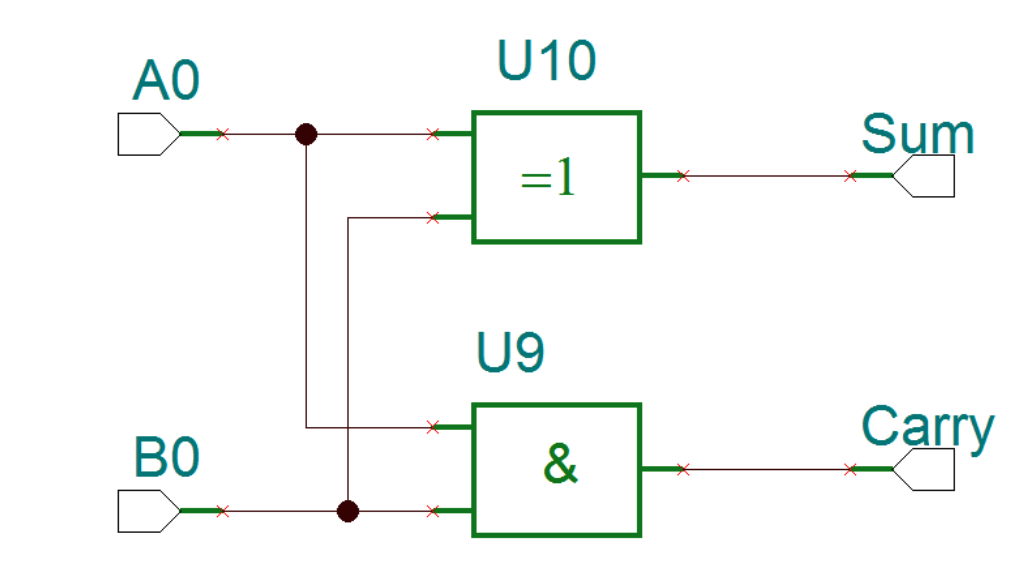
\includegraphics[height=30mm]{images/1bitadd.png}
\end{minipage}
\hfill
\\
\\
\begin{minipage}{1\linewidth}
	\begin{tabular}{| c | c | c | c|}
		\hline
		A0 & B0 & Sum & Carry \\
		\hline
		0 & 0 & 0 & 0 \\
		0 & 1 & 1 & 0 \\
		1 & 0 & 1 & 0 \\
		1 & 1 & 0 & 1 \\
		\hline
	\end{tabular} \\
\end{minipage}
\\
\\
\begin{minipage}{0.55\linewidth}
	\begin{tabular}{c c c c c c}
		  & 0 & 1 & 1 & 1 & \\
		+ & 0 & 1 & 0 & 1 & \\
		0 & 1 & 1 & 1 &   & Carry \\
		\hline
		0 & 1 & 1 & 0 & 0 & Sum \\
	\end{tabular} \\
\end{minipage}
\hfill
\begin{minipage}{0.35\linewidth}
	Sum = A0 \$ B0 \\
	Carry = A0 \& B0
\end{minipage}

\subsection{1-Bit Voll Addierer}
Addition mit Carry In. \\
\begin{minipage}{1\linewidth}
	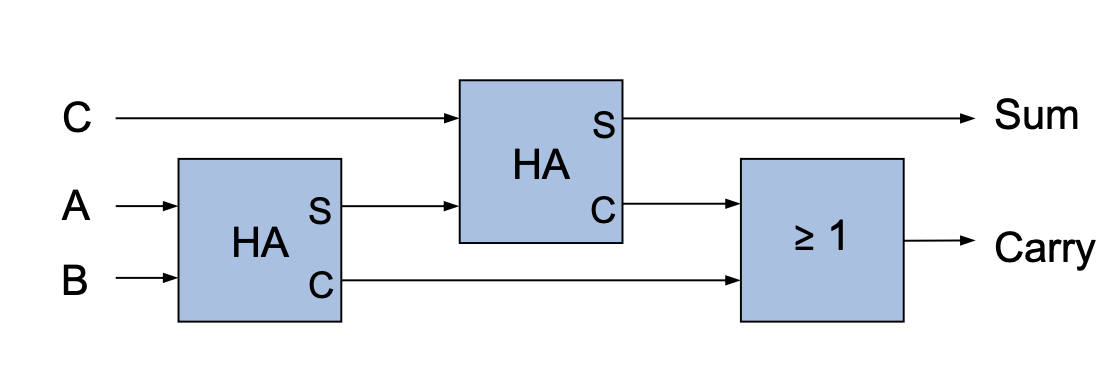
\includegraphics[height=20mm]{images/1bitvoll.png}
\end{minipage}
\hfill
\\
\\
\begin{minipage}{1\linewidth}
	\begin{tabular}{| c | c | c || c| c |}
		\hline
		C & A & B & Sum & Carry \\
		\hline
		0 & 0 & 0 & 0 & 0 \\
		0 & 0 & 1 & 1 & 0 \\
		0 & 1 & 0 & 1 & 0 \\
		0 & 1 & 1 & 0 & 1 \\
		1 & 0 & 0 & 1 & 0 \\
		1 & 0 & 1 & 0 & 1 \\
		1 & 1 & 0 & 0 & 1 \\
		1 & 1 & 1 & 1 & 1 \\
		\hline
	\end{tabular} \\
\end{minipage}


\subsection{4-Bit Addierer}
\begin{minipage}{1\linewidth}
	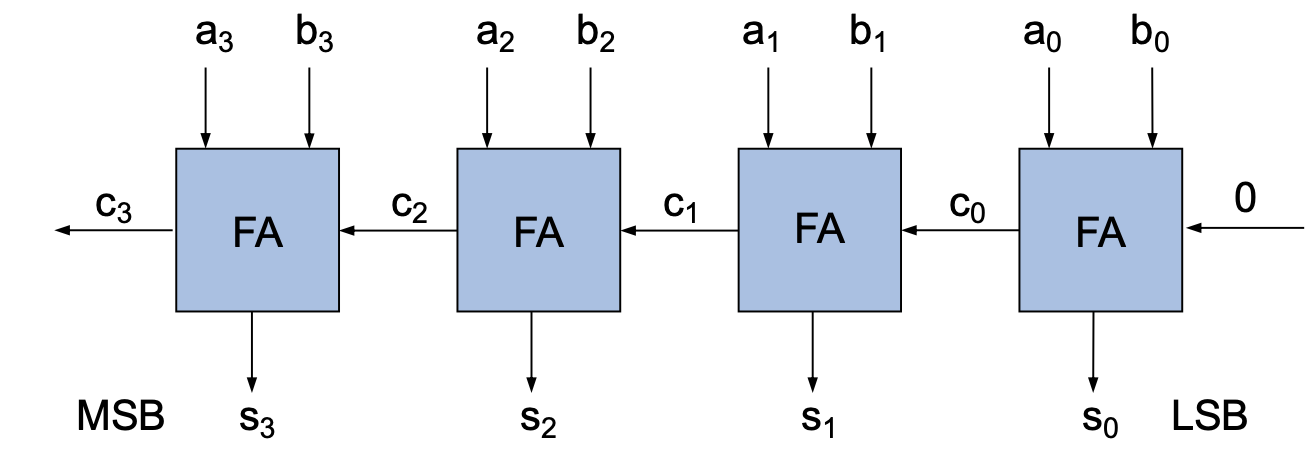
\includegraphics[height=20mm]{images/4bitadd.png}
\end{minipage}
\hfill
\\
\\
\begin{minipage}{1\linewidth}
	\begin{tabular}{| c | c | c || c| c |}
		\hline
		$C_i-1$ & $A_i$ & $B_i$ & $S_i$ & $C_i$ \\
		\hline
		0 & 0 & 0 & 0 & 0 \\
		0 & 0 & 1 & 1 & 0 \\
		0 & 1 & 0 & 1 & 0 \\
		0 & 1 & 1 & 0 & 1 \\
		1 & 0 & 0 & 1 & 0 \\
		1 & 0 & 1 & 0 & 1 \\
		1 & 1 & 0 & 0 & 1 \\
		1 & 1 & 1 & 1 & 1 \\
		\hline
	\end{tabular} \\
\end{minipage}


	\section{Sequentielle Logik}
\subsection{Abgrenzung zur Kombinatorischen Logik}
\begin{center}
    \begin{minipage}[t]{0.45\linewidth}
        \paragraph{Kombinatorische Schaltung}
        Output hängt von Inputs und Verknüpfungen ab.
	Das System hat keinen Speicher.
    \end{minipage}
    \hfill
    \begin{minipage}[t]{0.45\linewidth}
        \paragraph{Sequentielle Schaltung}
        Output hängt vom Zustand ab.
	Benötigt einen Speicher.
	Die Speicher-Ausgänge sind oft rückgekoppelt.
    \end{minipage}
\end{center}
\subsection{D-Flip-Flop}
\begin{minipage}{0.45\linewidth}
	\begin{center}
		
\includegraphics[width=0.5\linewidth]{images/dflip.png}
	\end{center}
\end{minipage}
\begin{minipage}{0.45\linewidth}
	Wert am Eingang D wird gespeichert und an den Ausgang Q übertragen, wenn C von 0 auf 1 wechselt.
\end{minipage}
\begin{center}
\begin{equation*}
	Q_{n+1} = D \quad \text{wenn} \quad CLK 0 \rightarrow 1
\end{equation*}
	$n$ Flip-Flops können $2^n$ Zustände annehmen.
\end{center}

\subsection{Clock Signal}
	\begin{minipage}{0.45\linewidth}
		\begin{center}
            	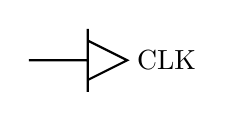
\begin{tikzpicture}
                	\draw[thick] (-0.75, 0) -- (0,0)
                    	(0,0.4) -- (0,-0.4)
                    	(0,0.25) -- (0.5,0) -- (0,-0.25);
                	\node[] at (1, 0) {CLK};
            	\end{tikzpicture}
        	\end{center}
        Input beim Übergang von \emph{$0 \rightarrow 1$} von CLK wirksam.
        \begin{center}
		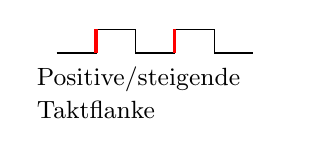
\begin{tikzpicture}
                	\draw (0,0) -- (0.5, 0) -- (0.5, 0.3) -- (1, 0.3) -- (1, 0) -- (1.5, 0) -- (1.5, 0.3) -- (2, 0.3) -- (2, 0) -- (2.5, 0);
                	\draw[very thick, red] (0.5, 0) -- (0.5, 0.3) (1.5, 0) -- (1.5, 0.3);
                	\node[text width = 30mm] at (1.25, -0.5) {\small Positive/steigende Taktflanke};
            	\end{tikzpicture}
        \end{center}
    	\end{minipage}
    	\hfill
    	\begin{minipage}{0.45\linewidth}
        	\begin{center}
            	
\begin{tikzpicture}
                	\draw[thick] (-0.75, 0) -- (0,0)
                    	(0,0.4) -- (0,-0.4)
                    	(0,0.25) -- (0.5,0) -- (0,-0.25);
                	\draw[thick, fill = white] (-0.1,0) circle [radius = 0.75mm];
                	\node[] at (1, 0) {CLK};
            	\end{tikzpicture}
        	\end{center}
        	Input beim Übergang von \emph{$1 \rightarrow 0$} von CLK wirksam.
        	\begin{center}
            		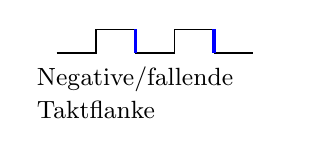
\begin{tikzpicture}
                		\draw (0,0) -- (0.5, 0) -- (0.5, 0.3) -- (1, 0.3) -- (1, 0) -- (1.5, 0) -- (1.5, 0.3) -- (2, 0.3) -- (2, 0) -- (2.5, 0);
                		\draw[very thick, blue] (1, 0.3) -- (1, 0) (2, 0.3) -- (2, 0);
                		\node[text width = 30mm] at (1.25, -0.5) {\small Negative/fallende Taktflanke};
            		\end{tikzpicture}
        	\end{center}
    	\end{minipage}

\subsection{Frequenzteiler}
Kaskadieren von T-Flipflops führt zu einer Frequenzreduktion von CLK um den Faktor 2.
\begin{center}
    \begin{minipage}{0.55\linewidth}
        \begin{circuit}[0.25]
            \ctikzset{multipoles/flipflop/clock wedge size=0.5}
            \node[tFfmin] (t1) {};
            \node[tFfmin, right = 6mm of t1] (t2) {};
            \node[tFfmin, right = 6mm of t2] (t3) {};
        
            \node[font = \footnotesize, left = 0.9mm of t1.pin 2] (clk) {\cirin{CLK}}; 
        
            \begin{pgfonlayer}{tl1}
                \node[circ] (nex1) at ($(t1.pin 6)!0.5!(t2.pin 1)$) {};
                \node[circ] (nex2) at ($(t2.pin 6)!0.5!(t3.pin 1)$) {};
            \end{pgfonlayer}
            \node[above = 4mm of nex1, font = \footnotesize] (q0) {$Q_0$};
            \node[above = 4mm of nex2, font = \footnotesize] (q1) {$Q_1$};
            \node[above = 4.5mm of t3.pin 6, font = \footnotesize] (q2) {$Q_2$};
        
            \draw (clk) -- (t1.pin 2);
            \draw (t1.pin 6) -- (nex1) |- (t2.pin 2);
            \draw (t2.pin 6) -- (nex2) |- (t3.pin 2);
            \draw (nex2) -- (q1);
            \path[draw] (nex1) -- (q0) node[midway, left, font = \footnotesize] {};  
            \path[draw] (t3.pin 6) -- (q2) node[midway, right, font = \footnotesize] {}; 
        \end{circuit}
    \end{minipage}
    \hfill
    \begin{minipage}{0.4\linewidth}
        \begin{center}
            \begin{tikzpicture}
                \coordinate[label = {[font = \footnotesize]180:\cirin{CLK}}](clk) at (0,0.5);
                \coordinate[label = {[font = \footnotesize]180:$Q_0$}](q1) at (0,0);
                \coordinate[label = {[font = \footnotesize]180:$Q_1$}](q2) at (0,-0.5);

                \draw[thick] (clk) --++(0:0.4) --++(90:0.2) coordinate(f1t) --++(0:0.4) --++(270:0.2) --++(0:0.4) --++(90:0.2) coordinate(f2t) --++(0:0.4) --++(270:0.2) --++(0:0.4) --++(90:0.2)coordinate(f3t) --++(0:0.05);
                \draw[thick] (q1) --++(0:0.4) --++(90:0.2) --++(0:0.8) --++(270:0.2)coordinate(f2b) --++(0:0.8) --++(90:0.2) --++(0:0.05);
                \draw[thick] (q2) --++(0:0.4) coordinate(f1b) --++(90:0.2) --++(0:1.6) --++(270:0.2)coordinate(f3b) --++(0:0.05);

                \begin{pgfonlayer}{bg}
                    \fill[red!50, rounded corners = 2pt] ($(f1t) +(-0.1,0.1)$) rectangle ($(f1b) + (0.1, -0.1)$);
                    \fill[red!50, rounded corners = 2pt] ($(f2t) +(-0.1,0.1)$) rectangle ($(f2b) + (0.1, -0.1)$);
                    \fill[red!50, rounded corners = 2pt] ($(f3t) +(-0.1,0.1)$) rectangle ($(f3b) + (0.1, -0.1)$);
                \end{pgfonlayer}
            \end{tikzpicture}
        \end{center}
    \end{minipage}
\end{center}

\subsection{Arten von Sequentiellen Schaltungen}
\subsubsection{Counter}
\begin{itemize}
	\item Einfache Form der sequentiellen Logik (endlicher Zustandsautomat).
	\item Zustandswechsel bei steigender Taktflanke.
	\item Die Reihenfolge der Zustände kann nicht von aussen beeinflusst werden.
	\item Die Ausgänge hängen nur vom internen Zustand ab.
\end{itemize}
\begin{center}
	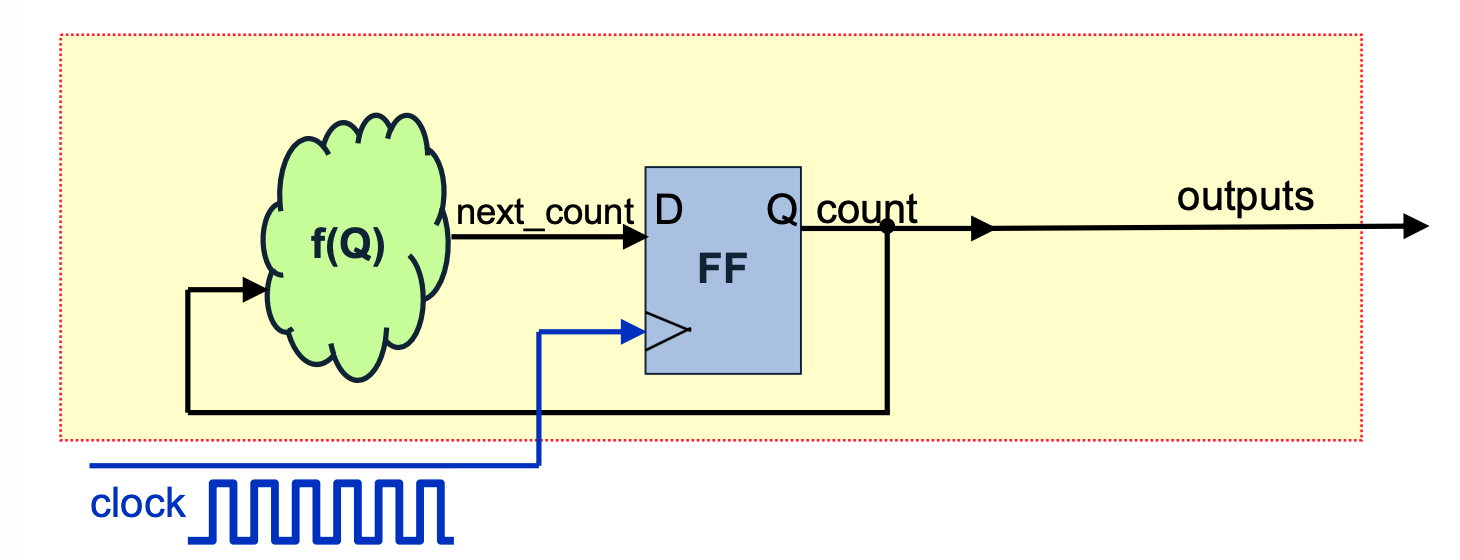
\includegraphics[width=1\linewidth]{images/counter.png}
\end{center}
\subsubsection{Finite State Machine}
\begin{itemize}
	\item Enthält Speicher.
	\item Der Ausgang ist abhängig vom Input und dem Status des Speichers.
	\item Der FF-Ausgangswert entspricht dem Zustand des Automaten.
	\item Bei jedem Takt-Signal (Clock) wird der Speicher neu geladen.
\end{itemize}
\begin{center}
	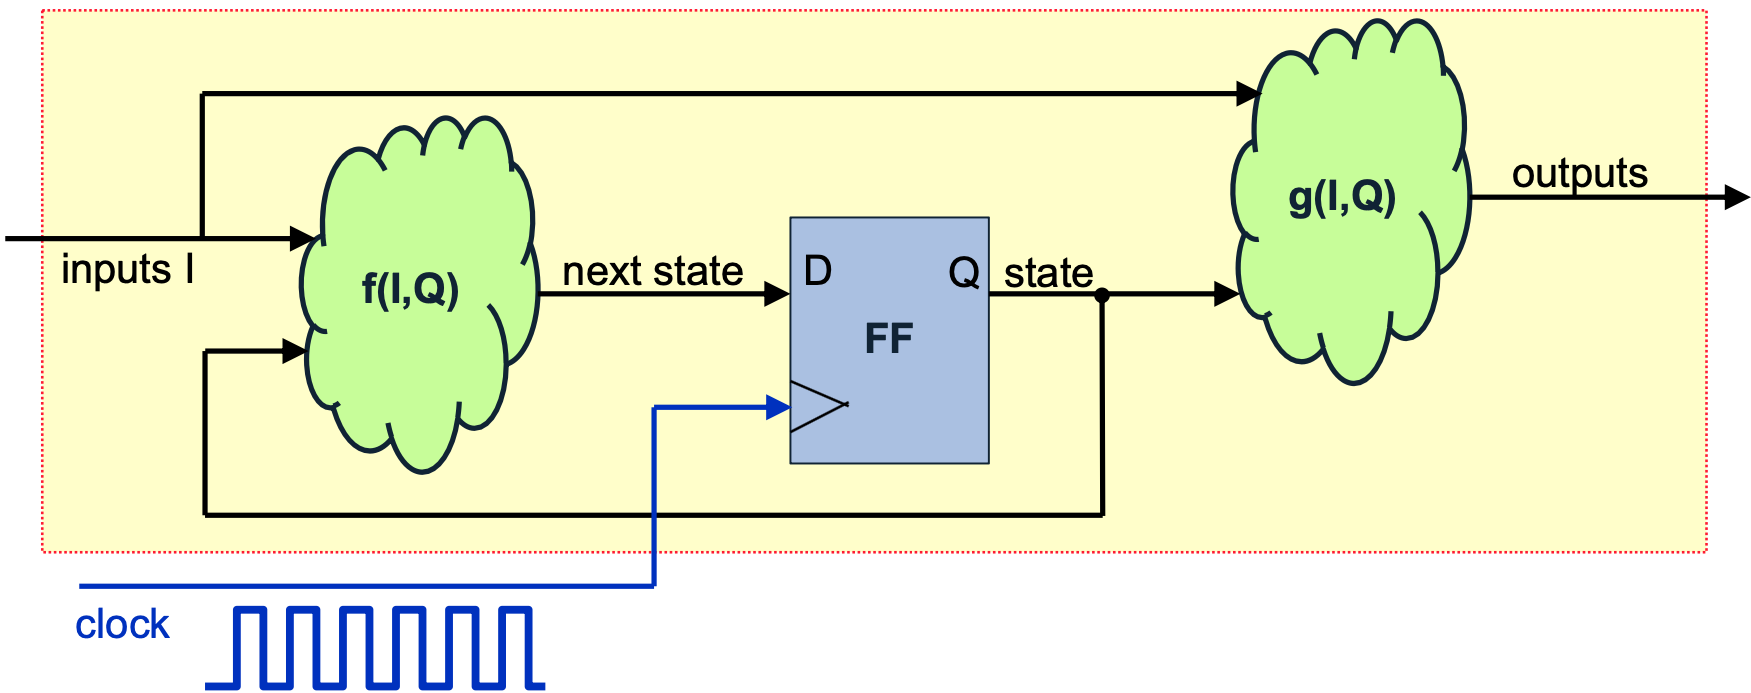
\includegraphics[width=1\linewidth]{images/FSM.png}
\end{center}
\subsubsection{Shift Register}
\begin{itemize}
	\item Enthält mehrere in Reihe geschaltete FFs.
	\item Die Eingänge können seriell oder parallel sein.
	\item Die Ausgänge können seriell oder parallel sein.
	\item Es kann Rückkopplungen enthalten oder nicht.
\end{itemize}
\begin{center}
	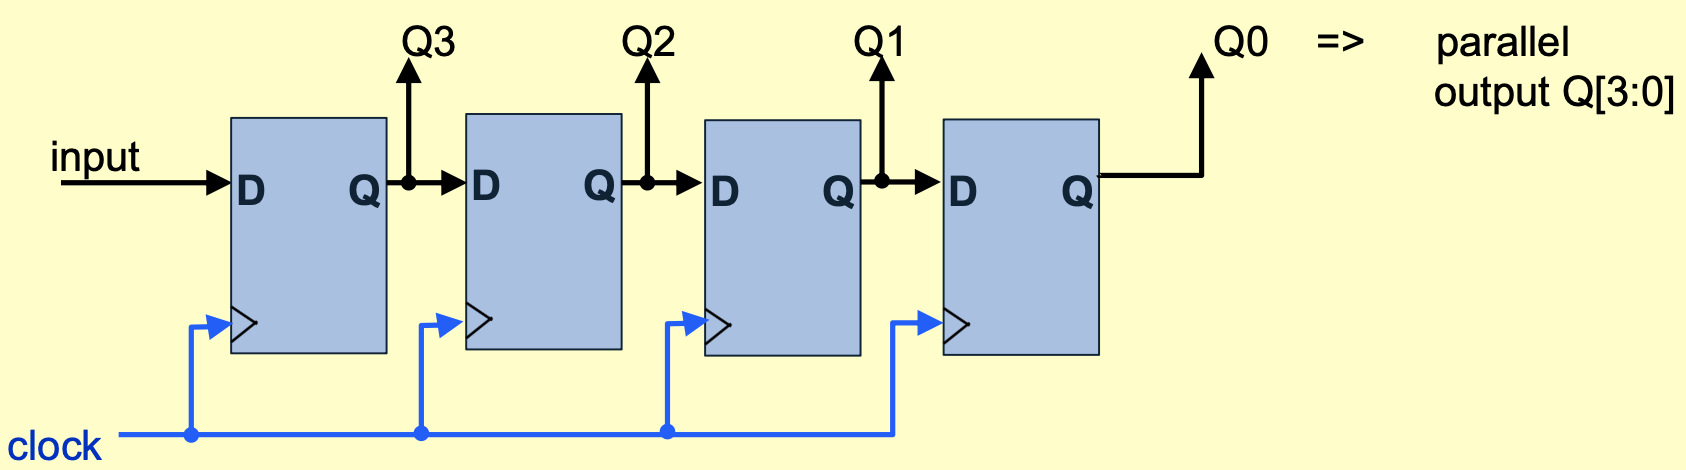
\includegraphics[width=1\linewidth]{images/shiftregister.png}
\end{center}

\subsection{Register}
\subsubsection{Parallel Register}
\begin{itemize}
	\item Ein- und Ausgänge sind parallel.
	\item Beispiel dafür: 8-bit Register.
	\item Inputs \quad in7 - in0 -> Werden bei steigender Flanke gespeichert.
	\item Outputs \quad out7 - out0.
	\item Schnellster Speicher im Prozessor.
\end{itemize}
\begin{center}
	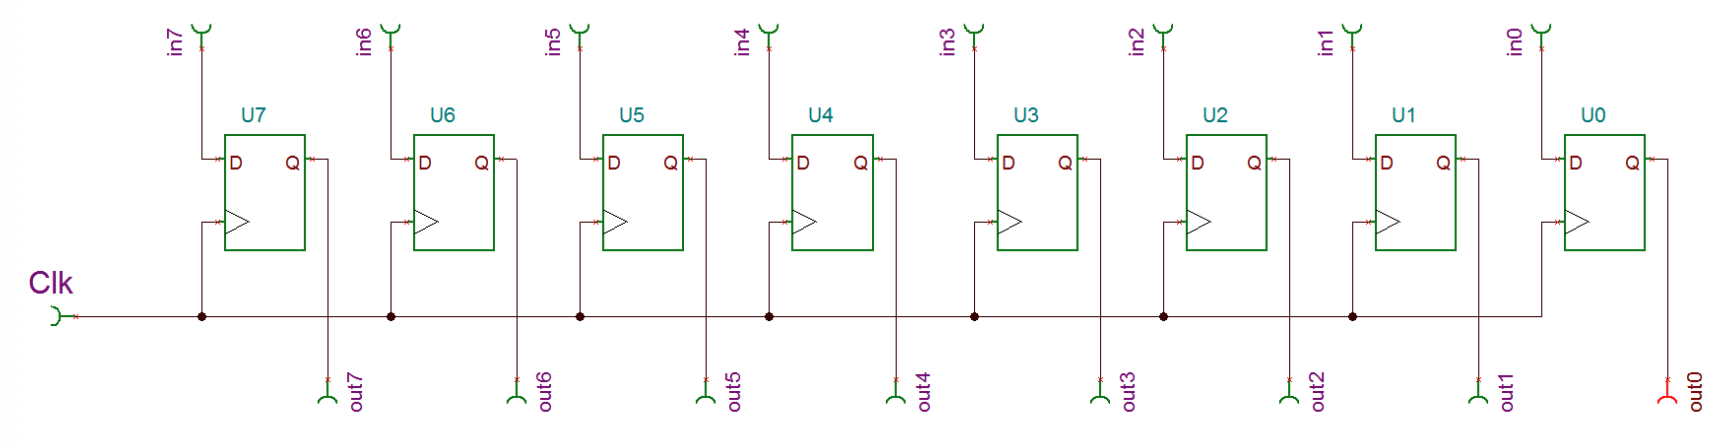
\includegraphics[width=1\linewidth]{images/8bitreg.png}
\end{center}
\subsubsection{Schieberegister}
\begin{itemize}
	\item Jeder Ausgang ist mit dem Eingang verbunden.
	\item Zustand des Ausgangs wird zum Eingang rübergeschoben bei jeder Flanke.
\end{itemize}
\begin{center}
	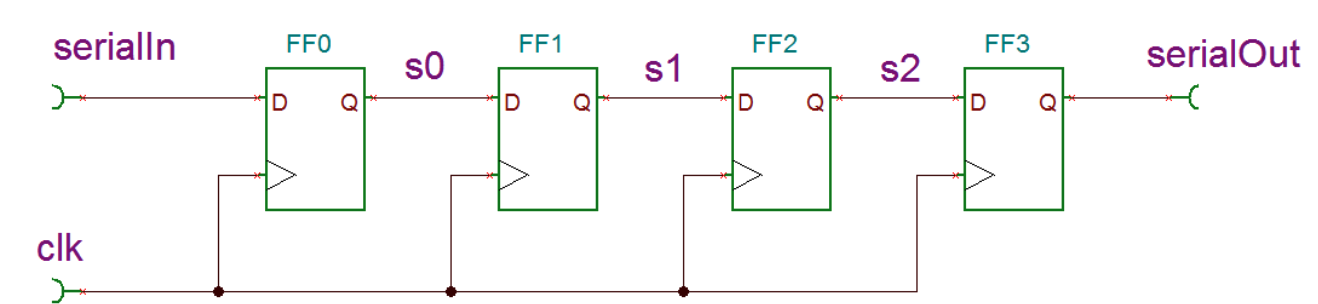
\includegraphics[width=1\linewidth]{images/schiebereg.png}
\end{center}
\begin{center}
	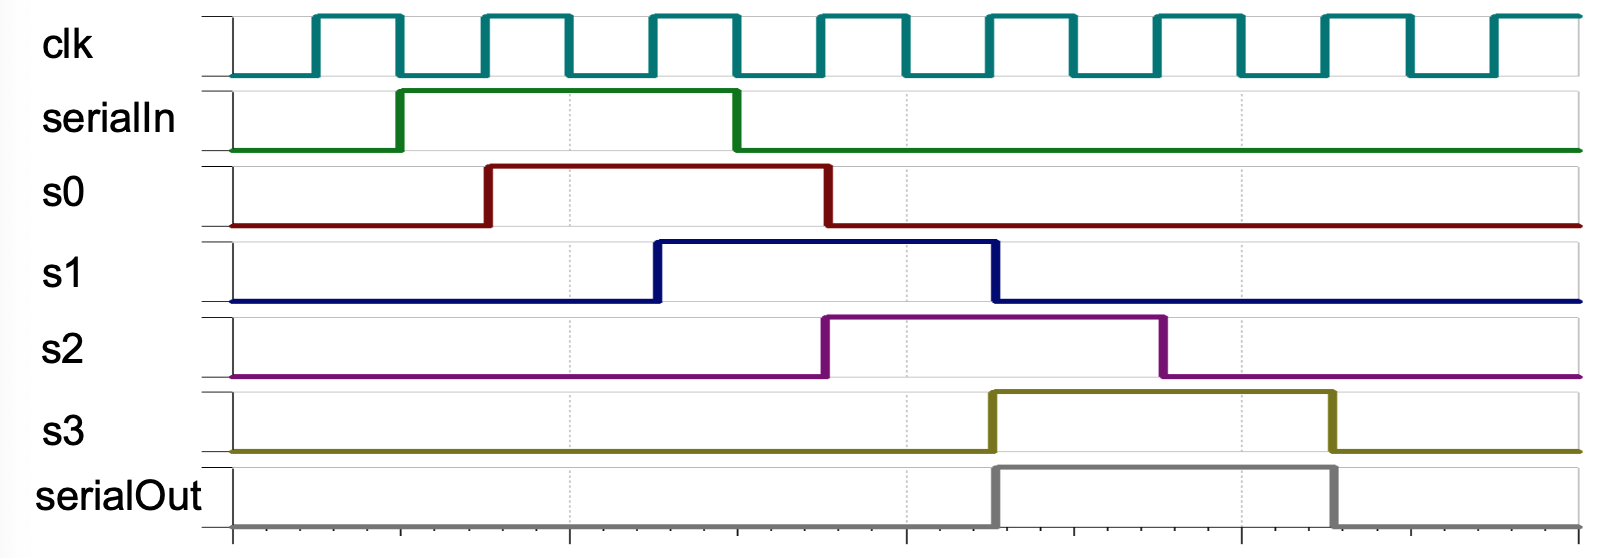
\includegraphics[width=1\linewidth]{images/schieberegtime.png}
\end{center}

\subsubsection{Beispiel für Zustandsdiagramm}
\begin{align*}
	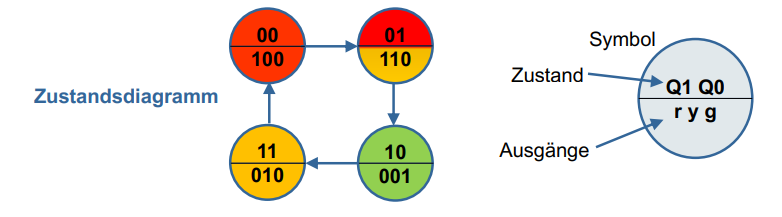
\includegraphics[width=1\linewidth]{images/zustandsdiagramm.png}
\end{align*}
	\section{Zahlensysteme}
\subsection{Stellenwertsysteme}
\begin{center}
    \begin{minipage}{0.65\linewidth}
        \begin{center}
            \begin{tabular}{c l}
                $Z$ & zu berechnende positive Zahl\\
                $b$ & Basis von $Z$\\
                $a_i$ & Koeffizient
            \end{tabular}
        \end{center}
    \end{minipage}
    \hfill
    \begin{minipage}{0.3\linewidth}
        \begin{equation*}
            Z = \sum_{i=0}^{n} a_i \cdot b^i
        \end{equation*}
    \end{minipage}
\end{center}
\begin{flushleft}
    \begin{tabular}{l c l}
        Dezimal & $10$ & $a_i \in \{0, 1, \dots, 9\}$\\
        Dual/Binär & $2$ & $a_i \in \{0, 1\}$\\
        Oktal & $8$ & $a_i \in \{0, 1, \dots, 7\}$\\
        Hexa & $16$ & $a_i \in \{0, 1, \dots, 9, A, B, C, D, E, F\}$\\
    \end{tabular}
\end{flushleft}
\begin{minipage}{0.3\linewidth}
	\subsubsection{Binärsystem}
	\begin{itemize}
		\item Index b
		\item In Java \texttt{0b}: \texttt{0b0010 0000}
	\end{itemize}
\end{minipage}
\hfill
\begin{minipage}{0.5\linewidth}
	\subsubsection{Hexadezimalsysem}
	\begin{itemize}
		\item Umfasst 16 Werte
		\item Index h
		\item In Java \texttt{0x}: \texttt{0xAF3C}
	\end{itemize}
\end{minipage}
\subsection{Umwandlung Zahlensysteme}
	Es gilt: $Z = a_n \cdot b^n ... + a_3 \cdot b^3 + a_2 \cdot b^2 + a_1 \cdot b^1 + a_0 \cdot b^0$ \\
	Wobei $Z$ den gegebenen Wert in einem Zahlensystem der Basis $b$ darstellt. \\
	Beispiel: $1000_d$ in hexadezimal
\subsubsection{Binär zu Dezimal}
\begin{center}
    \begin{tabular}{c|c|c|c|c|c|c|c}
        $2^7$ & $2^6$ & $2^5$ & $2^4$ & $2^3$ & $2^2$ & $2^1$ & $2^0$\\
        $128$ & $64$ & $32$ & $16$ & $8$ & $4$ & $2$ & $1$
    \end{tabular}
\end{center}
\begin{center}
    \begin{tabular}{c|c|c|c}
        $2^{-1}$ & $2^{-2}$ & $2^{-3}$ & $2^{-4}$\\
        $0.5$ & $0.25$ & $0.125$ & $0.0625$
    \end{tabular}
\end{center}

\subsubsection{Binär zu Hex}
\begin{center}
    \begin{tabular}{c c||c c||c c||c c}
        $0000$ & $0$ & $0100$ & $4$ & $1000$ & $8$ & $1100$ & $C$\\
        $0001$ & $1$ & $0101$ & $5$ & $1001$ & $9$ & $1101$ & $D$\\
        $0010$ & $2$ & $0110$ & $6$ & $1010$ & $A$ & $1110$ & $E$\\
        $0011$ & $3$ & $0111$ & $7$ & $1011$ & $B$ & $1111$ & $F$\\
    \end{tabular}
\end{center}

\subsubsection{Beispiel: Hexadezimal zu Dezimal}
\begin{enumerate}
    \item Umwandlung in Binär als Zwischenschritt. Dazu Tabelle verwenden.
    \[
        A23_{16} = 1010 0010 0011_2
    \]
    \item Umwandlung von Binär in Dezimal mittels 2er Potenzen
    \[
        2^{11}+2^9+2^5+2^1+2^0 = 2595_{10}
    \] 
    \item Bei einem signed Byte muss der Binärzahl zuerst ein Bit subtrahiert werden (Zweierkomplement bilden, dann addieren), dann invertiert. Danach die Zahl in Dezimal umwandeln und schliesslich ein Minus vor der Zahl setzen.
\end{enumerate}

\subsubsection{Modulare Arithmetik}
Falls eine Aufgabe mit Modulo kommt, letzte Ziffern anschauen und dadurch teilbarkeit bestimmen.

\begin{minipage}[t]{0.4\linewidth}
\subsubsection*{Horner-Schema}
	\begin{align*}
		1000 : 16 &= 62 \text{ Rest: }  8 \rightarrow 8\\
		62 : 16 &=  3 \text{ Rest: } 14 \rightarrow E\\
		3 : 16 &=  0 \text{ Rest: } 3 \rightarrow 3\\
		1000_10 &= 3E8_16
	\end{align*}

\subsubsection*{Zweierkomplement}
	\begin{align*}
		+2_d = &00000010_b\\
		\text{invertieren: } &11111101 \\
		\text{1 addieren: } &00000001 \\
		-2_d = &11111110_b
	\end{align*}
	
\subsubsection*{Einerkomplement}
	\begin{align*}
		0_d = &00000000_b\\
		\text{invertieren: } &11111111 \\
		\text{1 addieren: } &00000001 \\
		0_d = &00000000_b
	\end{align*}
\end{minipage}
\hfill
\begin{minipage}[t]{0.45\linewidth}
\subsubsection*{Kommastellen}
	\begin{align*}
		26.6875_d &= 26_d + 0.6876_d \\
		\\
		26_d : 2 &= 13 \text{ Rest: } 0 \\
		13_d : 2 &= 6 \text{ Rest: } 1 \\
		6_d : 2 &= 0 \text{ Rest: } 0 \\
		3_d : 2 &= 0 \text{ Rest: } 1 \\
		1_d : 2 &= 0 \text{ Rest: } 1 \\
		\\
		0.6875_d \cdot 2 &= 0.3750 + 1 \\
		0.3750_d \cdot 2 &= 0.7500 + 0 \\
		0.7500_d \cdot 2 &= 0.5000 + 1 \\
		0.5000_d \cdot 2 &= 0.0000 + 1 \\
		\\
		26.6875_d &= 11010.1011_b
	\end{align*}
\end{minipage}
\subsubsection{Neuner, bzw. Zehnerkomplement}%
\label{ssub:neuner_bzw_zehnerkomplement}
Für das Neunerkomplement einer Dezimalzahl notiert man jeweils für jede Ziffer deren Unterschied zu 9. Für das Zehnerkomplement addiert man 1. Wenn man mittels Neunerkomplement Subtrahieren möchte, bildet man das Zehnerkomplement des Subtrahenden und addiert die Zahlen schliesslich. Der Übertrag wird dabei ignoriert.


\subsection{Endliche Zahlen}
\begin{tabular}{| c | c | c | c |}
	\hline
	Reg. & Bez. & Unsinged & Int \\
	\hline
	\hline
	4 Bit & Nibble & $0 ... 15_d$ & $-8 ... +7$ \\
	\hline
	8 Bit & Byte & $255_d$ & $-128$/$127$ \\
	\hline
	16 Bit & Word & $65535_d$ & $-32768$/$32767$ \\
	\hline
	32 Bit & d. Word & $4.29_d \cdot 10^9$ & $\pm 2.15 \cdot 10^9$ \\
	\hline
	64 Bit & l. Word & $1.84_d \cdot 10^{19}$ & $\pm 9.22 \cdot 10^{18}$ \\
	\hline
	128 Bit & d.l. Word & $3.40_d \cdot 10^{38}$ & $\pm 1.70 \cdot 10^{38}$ \\
	\hline
\end{tabular}

\subsection{Carry und Overflow}
\begin{itemize}
	\item \textit{Carry} bezeichnet übertrag bei Operation die die Grösse des Registers überschreitet.
	\item Übertrag nach unten wird als \textit{borrow} bezeichnet.
	\item Bei vorzeichenbehafteten Zahlen tritt der Sprung dort auf, wo MSB wechselt.
	\item Bei MSB = 0 ist Registerinhalt null oder positiv. Bei MSB = 1 ist die Zahl negativ.
	\item \textit{Overflow} = vorzeichenbehafteter Übertrag.
	\item Für Carry, Borrow und Overflow existiert ein Flag im Mikroprozessor.
\end{itemize}

\subsection{Addition und Subtraktion}
\begin{enumerate}
	\item Summanden untereinander auflisten.
	\item Summanden bitweise addieren, dabei Übertrag beachten.
	\item Bei der Subtraktion das Zweierkomplement bilden und schliesslich addieren.
	\item Übertrag von MSB ignorieren.
\end{enumerate}

\subsection{Multiplikation}
\begin{center}
    \begin{minipage}[t]{0.70\linewidth}
        \begin{enumerate}
            \item Bitweise Multiplikation des Multiplikanden $a$ mit $b_i$ des Multiplikator.
            \item Sukzessive Multiplikationen werden um ein Bit ($0$) nach links verschoben.
            \item Anzahl Nachkommabits ergibt sich aus der Summe der Anzahl Nachkommabits der Operatoren.
        \end{enumerate}
    \end{minipage}
    \hfill
    \begin{minipage}[t]{0.25\linewidth}
        \begin{align*}
            b_0 \cdot a&\\
            +b_1 \cdot a~0\\
            +b_2 \cdot a~0~0&\\
            +b_3 \cdot a~0~0~0&\\
            \hline
            =\text{Sum}&
        \end{align*}
    \end{minipage}
\end{center}

\subsection{Division}
\begin{center}
    \begin{minipage}{0.7\linewidth}
        \begin{enumerate}
            \item Identifiziere Teil des Divident $>$ Divisor (Unterblock). Für jede Stelle, sodass Divident $<$ Divisor, 0 in Quotient.
            \item Unterblock $-$ Divisor, 1 an Quotient anhängen, Rest behalten.
            \item An das Resultat der Subtraktion Bits des Dividenten anhängen. Wiederholen bis Subtraktion 0 ergibt.
        \end{enumerate}
    \end{minipage}
    \hfill
    \begin{minipage}{0.25\linewidth}
        \begin{adjustbox}{angle=90}
            \setlength{\tabcolsep}{0.3mm}
            \footnotesize
            \begin{tabular}{rcc|l}
                \multicolumn{4}{c}{${\color{darkgreen}11100}:0111 = {\color{blue}0100}$}\\
              \hline
              ${\color{darkgreen}1}$ & \% & $111 = {\color{blue}0}$ & $R={\color{pastelviolet!50!red} 1}$\\
              ${\color{pastelviolet!50!red} 1}{\color{darkgreen}1}$ & \% & $111 = {\color{blue}0}$ & $R={\color{pastelviolet!50!red}11}$\\
              ${\color{pastelviolet!50!red} 11}{\color{darkgreen}1}$ & \% & $111 = {\color{blue}1}$ & $R={\color{pastelviolet!50!red}000}$\\
              ${\color{pastelviolet!50!red} 000}{\color{darkgreen}0}$ & \% & $111 = {\color{blue}0}$ & $R={\color{pastelviolet!50!red}0000}$\\
              ${\color{pastelviolet!50!red} 0000}{\color{darkgreen}0}$ & \% & $111 = {\color{blue}0}$ & $R={\color{pastelviolet!50!red}00000}$\\
            \end{tabular}
        \end{adjustbox}
    \end{minipage}
\end{center}

	\section{Informationstheorie}

\subsection{Quellen-Modell}%
\label{sub:quellen_modell}
\begin{enumerate}
	\item Eine Datenquelle ist gibt zufällige Nachrichten $X_n$ aus, mit $k=0,1,2,...$.
	\item $X_0$ ist die Nachricht nach dem Start.
	\item $X_k$ ist eine beliebige Nachricht aus dem Nachrichtenstrom.
	\item $k$ sagt nichts über den Inhalt der Nachricht aus.
\end{enumerate}

\subsection{Typen von Datenquellen}%
\label{sub:typen_von_datenquellen}
\subsubsection{Discrete Memoryless Source (DMS)}%
\label{ssub:discrete_memoryless_source_dms_}
\begin{enumerate}
	\item \textbf{Discrete:} Qulle liefert zeitlich einzelne Ereignisse.
	\item \textbf{Memoryless: } Quelle erinnert sich beim Produzieren eines Ereignisses nicht an
		die Vorgeschichte. D.h. Symbole sind statistisch unabhängig voneinander.
\end{enumerate}
\subsubsection{Binary Memoryless Source}%
\label{ssub:binary_memoryless_source}
	DMS, die lediglich zwei verschiedene Ereignisse erzeugt.

\subsection{Informationsgehalt}%
\label{sub:informationsgehalt}
\subsubsection{Informationsgehalt von Ereignissen mit gleichen Wahrscheinlichkeiten}%
\begin{enumerate}
	\item Werden $F$ Ja/Nein Antworten benötigt, um zu einer Antwort zu gelangen, so muss eine Nachricht
	$x_n$, welche diese Antwort als Ganzes erhält, gleich viel Information $I(x_n)$ enthalten; also $F$ Bit.
	\item Mit $F$ Fragen können maximal $N$ Fragen eingegrenzt werden ($2^F \geq N$)
	\item $\rceil F = \log{2}{N} \lceil$ (Bit)
	\item $I(x_n) = \log{2}{N} (Bit)$
	\item Je mehr Fälle, desto seltener tritt ein Ereignis ein.
	\item Je seltener ein Ereignis, desto höher sein Informationsgehalt.
	\item Wenn alle Ereigniswerte $x_n$ die gleiche Auftretenswahrscheinlichkeit $P(x_n)$ haben, gilt: \\
		$P(x_n) = \frac{1}{N} \implies N=\frac{1}{P(x_n)}$
	\item Für den Informationsgehalt eines Ereignisses folgt: \\
		$I(x_n) = \log{2}{\frac{1}{P(x_n)}}$
\end{enumerate}

\subsubsection{Auftretenswahrscheinlichkeit $P(x_n)$}%
\begin{enumerate}
	\item $k(x_n)$ sei die absolute Häufigkeit von $x_n$ in den $K$ Ereignissen.
	\item Die Auftretenswahrscheinlichkeit ist dann: \\
		$P(x_n) = \frac{k(x_n)}{K}$
\end{enumerate}

\subsubsection{Grenzbetrachtung}%
\label{ssub:grenzbetrachtung}
\begin{enumerate}
	\item Ereignis das praktisch sicher eintritt: $P(x_n) \rightarrow 1$ \\
		$I_{min} = \lim_{P(x_n) \to 1} \log{2}{\frac{1}{P(x_n)} = 0}$
	\item Ereignis das sozusagen nie eintritt: $P(x_n)\rightarrow 1$ \\
		$I_{max} = \lim_{P(x_n) \to 0} \log{2}{\frac{1}{P(x_n)}=0}$
\end{enumerate}

\subsection{Entropie}%
\label{sub:entropie}
\begin{equation*}
	H(X) = \sum^{N-1}_{n=0} P(x_n) \cdot \log{2}{\frac{1}{P(x_n)}} 
\end{equation*}

\subsubsection{Binäre, gedächtnislose Quelle}%
\label{ssub:binäre_gedächtnislose_quelle}
\begin{enumerate}
	\item Eine Binary Memoryless Source BMS kennt nur 2 Symbole.
	\item Daraus folgt, dass wenn $p$ die Auftretenswahrscheinlichkeit des einen Symbol ist, ist die
		Auftretenswahrscheinlichkeit des anderen Symbols $(1-p)$.
	\item Für die binäre Entropie $H_b$ gilt also: \\
		$H_b = p \cdot log{2}{\frac{1}{p}} + (1-p) \cdot log{2}{\frac{1}{1-p}}$
\end{enumerate}

\subsubsection{Entropie Eigenschaften}
\begin{enumerate}
	\item Eine Quelle $X$ liefere $N$ verschiedene Symbole $x_n$, die alle identische Wahrscheinlichkeiten
		$P(x_n)=\frac{1}{N}$ haben, dann gilt: \\
		$H(X)=\sum^{N-1}_{n=0}P(x_n) \cdot \log{2}{\frac{1}{P(x_n)}} = N \cdot \frac{1}{N} \cdot
		\log{2}{N} = \log{2}{N}$
	\item Minimale Entropie: Falls es am Ausgang einer Quelle $X$ ein Symbol $x_n$ gibt mit $P(x_n) = 1$, 
		so ist $H(X)=0$. Die minimale Entropie $H_{min}$ ist demnach: \\
		$H_{min} = 0$
	\item Maximale Entropie: Wenn $N$ die Anzahl möglicher Symbole einer Quelle $X$ ist, so gilt $0\leq H
		(X) \leq \log{2}{N}$. Die maximale Entropie $H_{max}$ ist demnach: \\
		$H_{max} = \log{2}{N}$
\end{enumerate}

	\section{Quellencodierung}
Ziel: Redundanz entfernen.
Die optimale binäre Codierung lässt sich durch Entropierechnung herausfinden.
\subsection{Redundanz}
Anteil in einer Codierung, die keine Information trägt. \\
Mittlere Länge einer Codierung:
\[L= \sum_{n=0}^{N=1} P(x_n)\cdot l_n\]
Redundanz:
\[R=L-H\]
\textbf{Beispiel: Packed BCD, Ziffern 0...9 codiert in 4 Bit}
\begin{enumerate}
    \item $P(x_{0...9}) = 0.1$
    \item Entropie, $H_{BCD} = 10 \cdot 0.1 \cdot \log_{2}{10} = 3.32$ Bit pro Symbol
    \item Code Länge, $L_{BCD} = 4$ Bit pro Symbol
    \item Redundanz, $R = L_{BCD} - H_{BCD} = 4 - 3.32 = 0.68$ Bit pro Symbol
\end{enumerate}

\subsubsection{Kompressionsrate}
Die Kompressionsrate $R$ ist der Quotient von komprimierten Bits durch originale Bits. Obwohl Kompressionsrate und Redundanz beide mit $R$ bezeichnet werden, haben diese Grössen nichts miteinander zu tun.

\subsubsection{Codes unterschiedlicher Länge}
Codes unterschiedlicher Länge sind möglich, Voraussetzung ist jedoch die Präfixfreiheit. D.h. kein Code bildet den Anfang eines anderen Codes.

\subsubsection{Theorem zur Quellencodierung}
\begin{enumerate}
    \item Solange die Redundanz R eines Codes grösser als null ist (L > H), kann verliustfrei komprimiert werden. Idealfall: L=H, bzw. R=0.
    \item Falls $R \leq 0$, so kann nur verlustbehaftet komprimiert werden.
\end{enumerate}

\subsection{Lauflängencodierung}
Ketten von identischen Zeichen werden zusammengefasst. RLE codiert runs wie folgt: (Marker, Anzahl, Zeichen)
\begin{enumerate}
    \item Als Marker wird ein selten genutzter Code verwendet. Hier A.
    \item Eine Zählerbreite in Bits wird so gewählt, dass Runs der typischen Länge damit erfasst werden können.
    \item Annahme: 2-Bit-Symbole und 6-Bit-Zähler: M+A+Z = 2+6+2 = 10 Bit.
    \item Beispiel:
    \[\mathtt{TERRRRRRRRRMAUIIIIIIIIIIIIIIIIIWQCSSSSSSSSSSL}=\]
    \[\mathtt{TEA09RMA01AUA17IWQCA10SL}\]
\end{enumerate}

\subsection{Huffman Codes}
\subsubsection{Verfahren}
\begin{enumerate}
    \item Ordne alle Symbole nach aufsteigenen Auftretenswahrscheinlichkeiten auf einer Zeile. Dies sind die Blätter des Huffman-Baums.
    \item Notiere unter jedes Blatt seine Wahrscheinlichkeit.
    \item Schliesse die beiden Blätter mit der kleinsten Wahrscheinlichkeit an einer gemeinsamen Astgabel an und ordne dem Ast die Summe der Wahrscheinlichkeiten der beiden Blätter zu.
    \item Wiederhole Punkt 3 mit Blättern und Ästen so lange, bis nur noch der Stamm des Baums übrig bleibt.
    \item Nun wird bei jeder Astgabel dem einen Zweig eine 0 und dem anderen eine 1 zugeordnet. (Die Zuordnung ist frei wählbar, muss aber über den ganzen Baum einheitlich sein).
    \item Nun werden auf dem Pfad vom Stamm zu jedem Blatt die Nullen und Einsen ausgelesen und von links nach rechts nebeneinander geschrieben. Dies sind die Huffman-Codeworte.
\end{enumerate}
\begin{align*}
    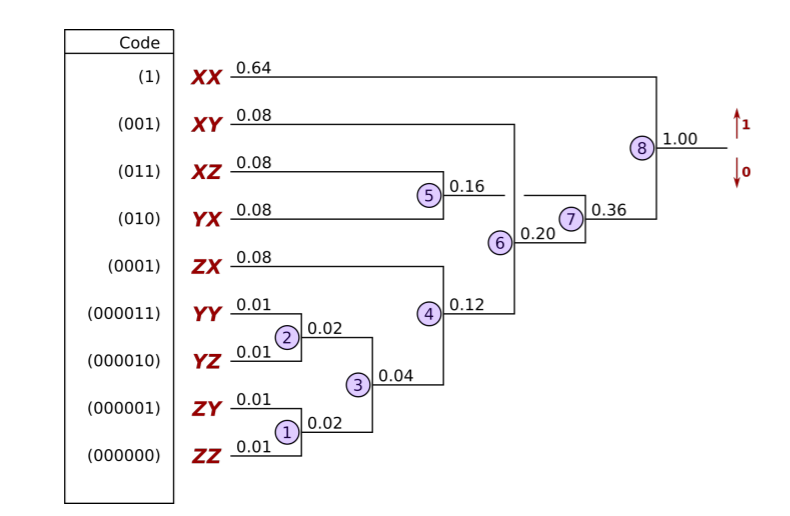
\includegraphics[width=1\linewidth]{images/huffman.png}
\end{align*}

\subsection{LZ77}
Alle Zeichen werden durch Token fixer Länge ersetzt. Token: (Offset, Länge, Zeichen)
\begin{align*}
    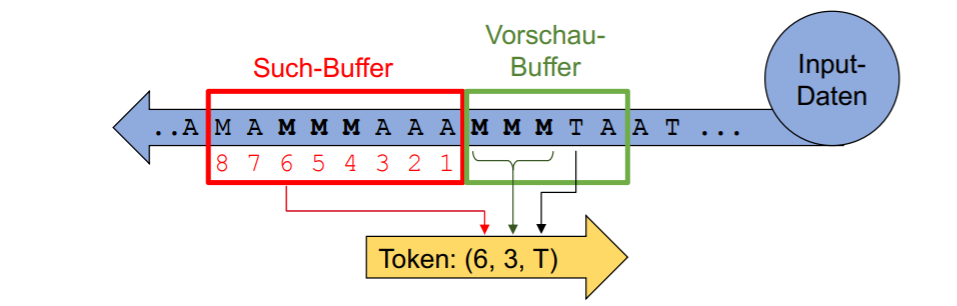
\includegraphics[width=1\linewidth]{images/lz77.png}
\end{align*}

\subsection{LZW}
\begin{enumerate}
    \item Statt einem Sliding Window wird ein Wörterbuch verwendet
    \item Der Index nummeriert die Einträge des Wörterbuchs
    \item Der String bildet den eigentlichen Eintrag
    \item Wörterbuch wird initialisiert mit den möglichen Zeichen resp. Byte-Werten (0..255). à Einzelne Zeichen sind im WB immer vorhanden.
    \item Token enthält nur den Index des schon bestehenden Eintrags im Wörterbuch, nicht aber das zusätzliche Zeichen. Token: (Index)
    \item Das neue Zeichen wird erst mit dem nächsten Token übermittelt (Überlappung)
\end{enumerate}
\textbf{Beispiel: } $\mathtt{A M A M M M A A A M M M T A A T ...}$
\begin{align*}
    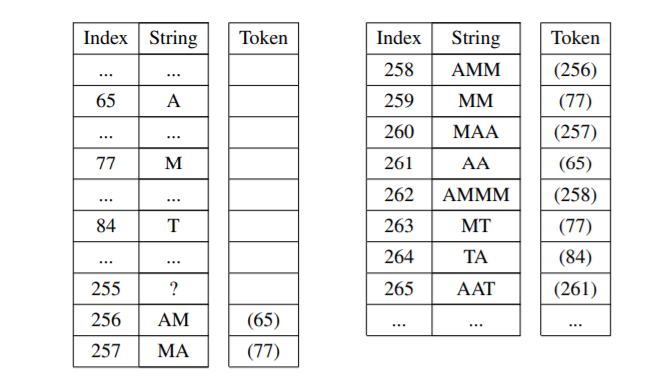
\includegraphics[width=1\linewidth]{images/lzw.png}
\end{align*}

\subsection{Bildkompression - JPEG}

\begin{center}
    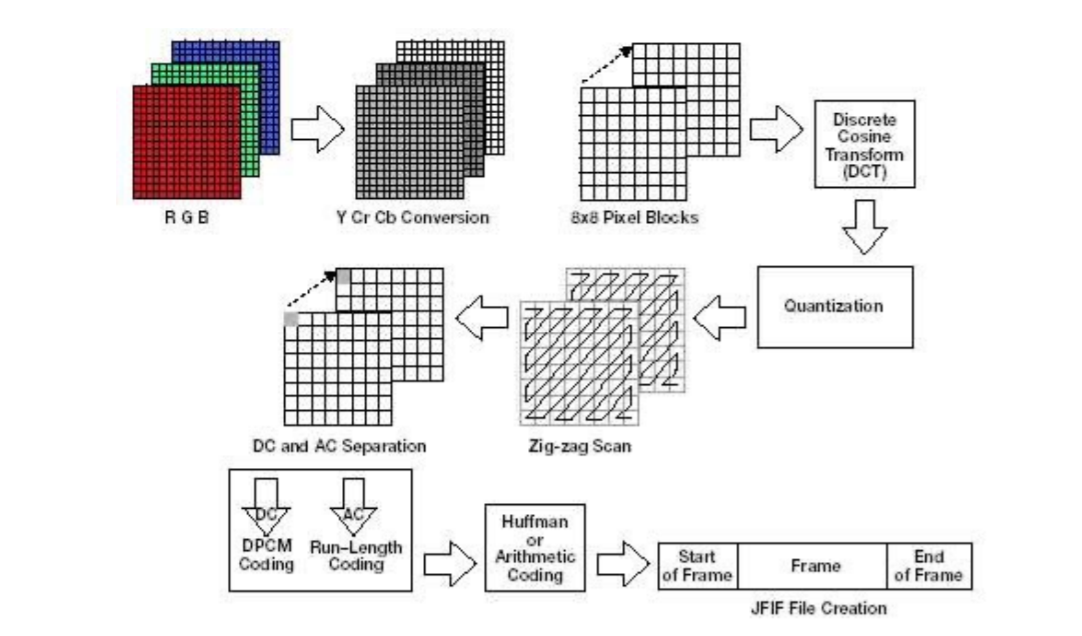
\includegraphics[width=1\linewidth]{images/verfahren.png}
\end{center}

\subsubsection{Kompressionsschritte}%

\begin{enumerate}
    \item Transformation Farbbilder RGB -> Luminanz, Chrominanz
    \item Downsampling der beiden Chrominanz-Komponenten
    \item Pixel-Gruppierung Farbkomponenten in 8x8 Blöcke
    \item Direkte Cosinus Transformation (8x8 DCT)
    \item Individuelle Quantisierung einzelner Frequenzkomponenten
    \item Entropy-Coding der quantisierten Frequenzkomponenten
    \item Erstellen von Header mit JPEG-Parametern
\end{enumerate}

\subsubsection{Luminanz und Chrominanz Farbmodell}

\begin{center}
    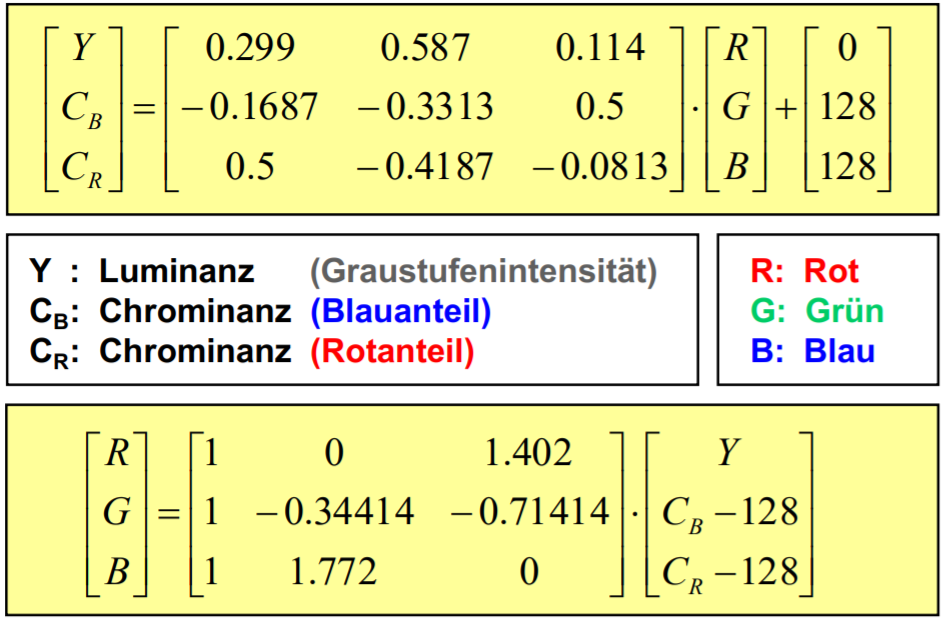
\includegraphics[width=1\linewidth]{images/lumchrom.png}
\end{center}

\subsubsection{Downsampling}

Bei Downsampling werden in beiden Chrominanz-Ebenen in der Horizontalen oder Vertikalen mehrere Pixel zusammengefasst. \\
\textbf{Beispiel: } 4:2:0, 4 bezeichnet hier die Breite des Referenzblocks, 2 bezeichnet wie viele Pixel nach dem Downsampling auf der ersten Zeile und 0 auf der zweiten Zeile vorliegen.
\begin{center}
    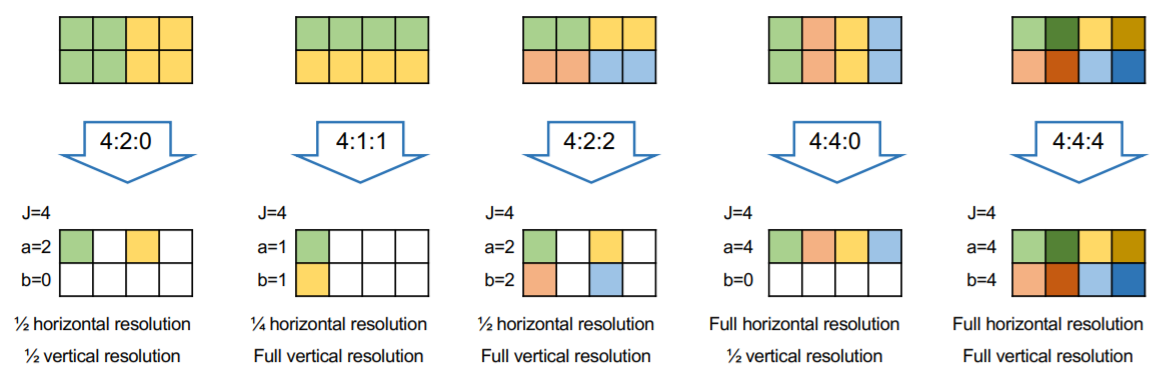
\includegraphics[width=1\linewidth]{images/downsampling.png}
\end{center}

\subsubsection{JPEG Blockverarbeitung}

\begin{center}
    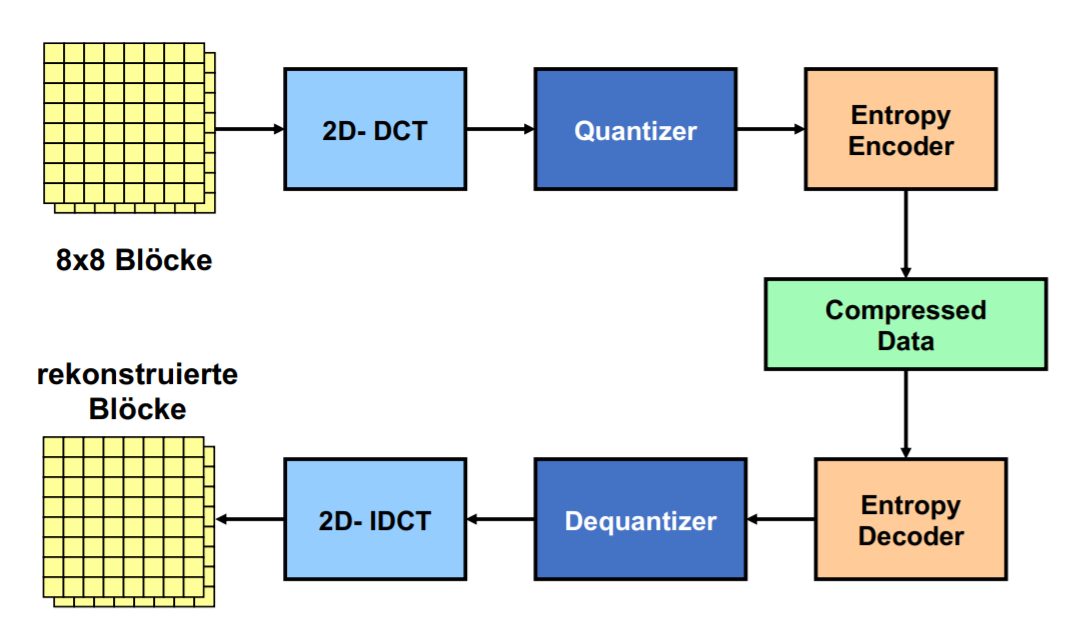
\includegraphics[width=1\linewidth]{images/blockverarbeitung.png}
\end{center}

\subsubsection{DCT Basisfunktion}

\begin{center}
    
\includegraphics[width=0.6\linewidth]{images/dct.png}
\end{center}

\begin{center}
    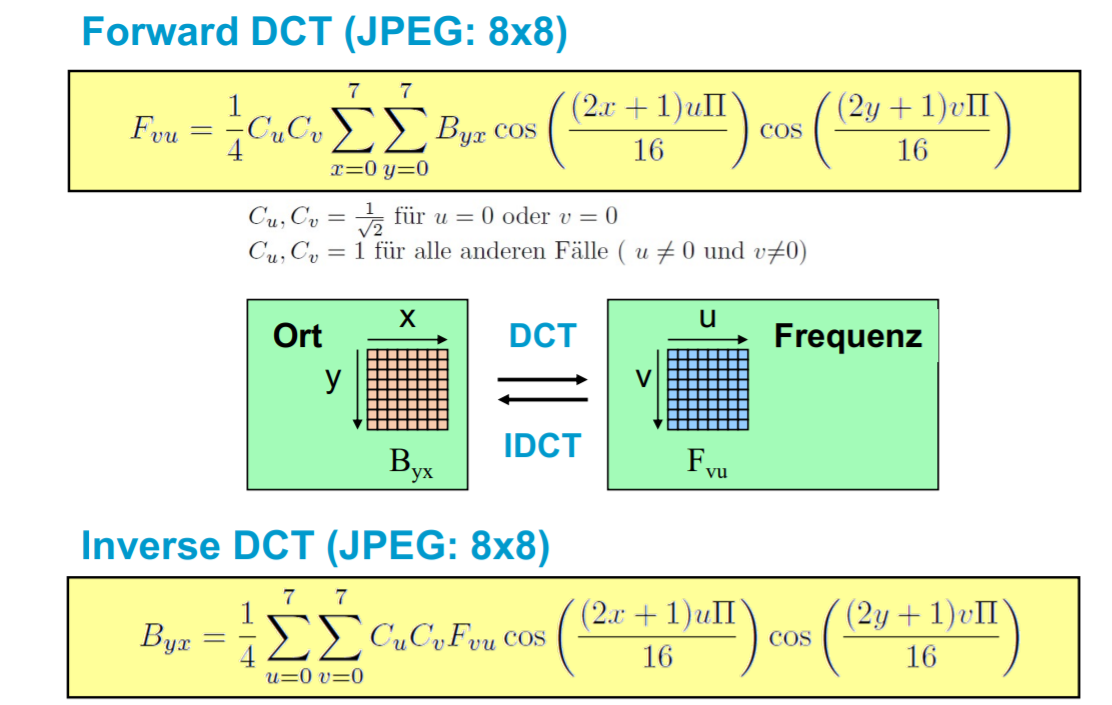
\includegraphics[width=1\linewidth]{images/dctfunction.png}
\end{center}

\begin{center}
    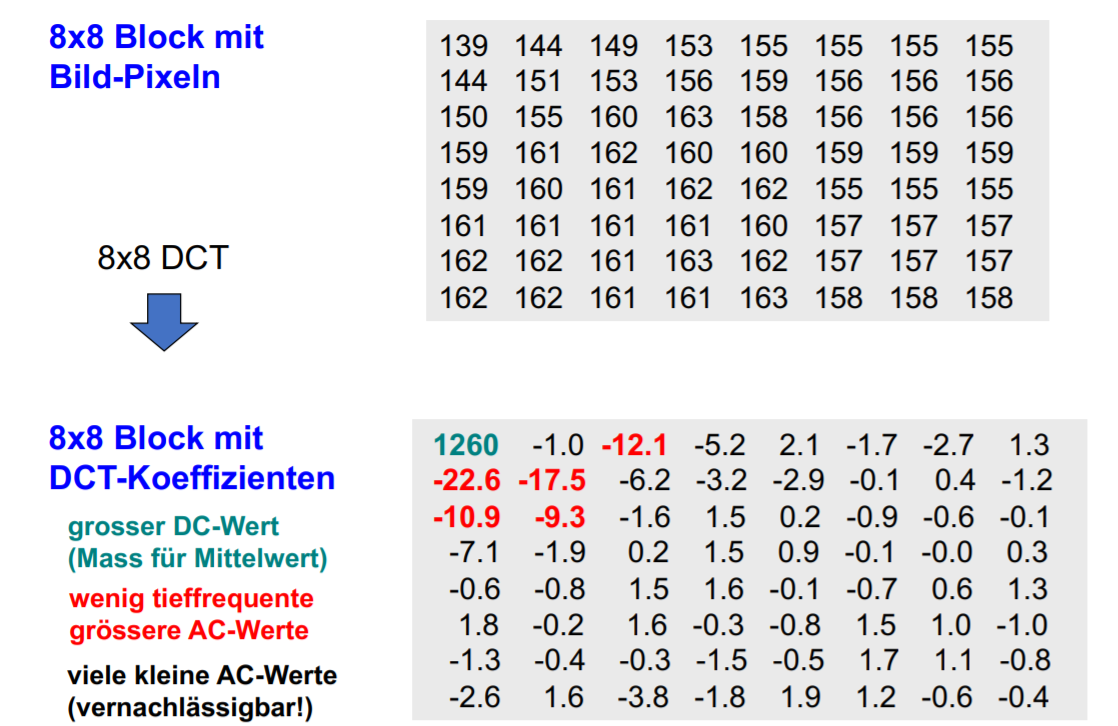
\includegraphics[width=1\linewidth]{images/dctblock.png}
\end{center}

\subsubsection{Quantisierung}%

\begin{center}
    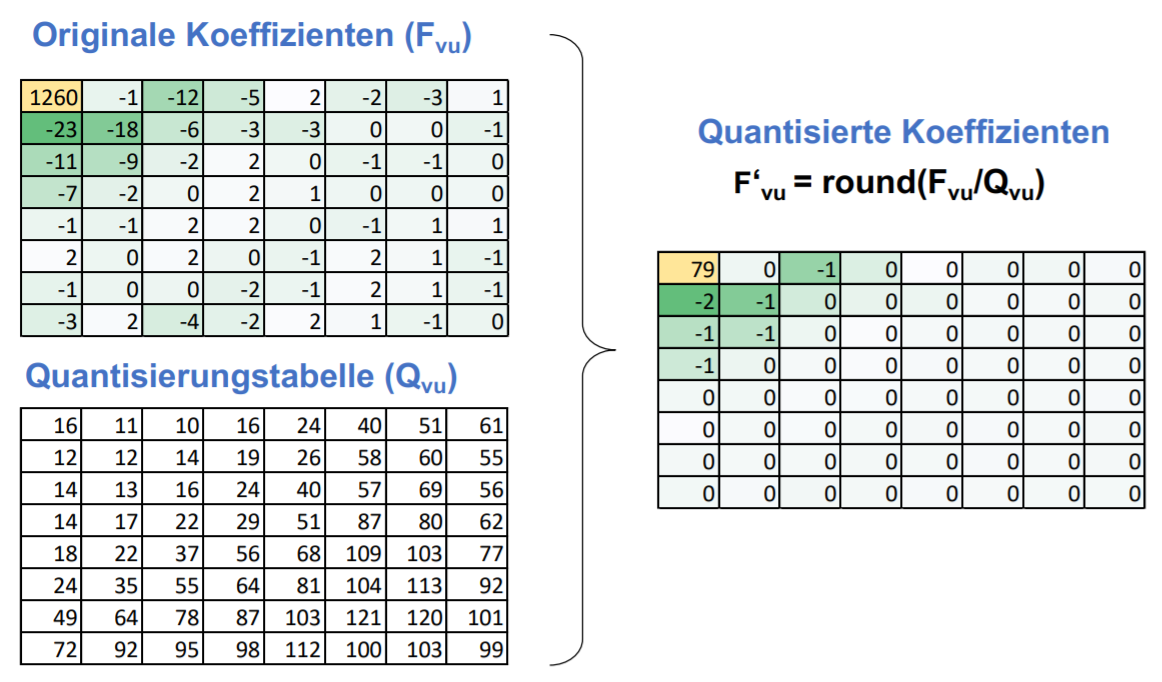
\includegraphics[width=1\linewidth]{images/quantisierung.png}
\end{center}

\subsubsection{Entropy Encoder}

\begin{center}
    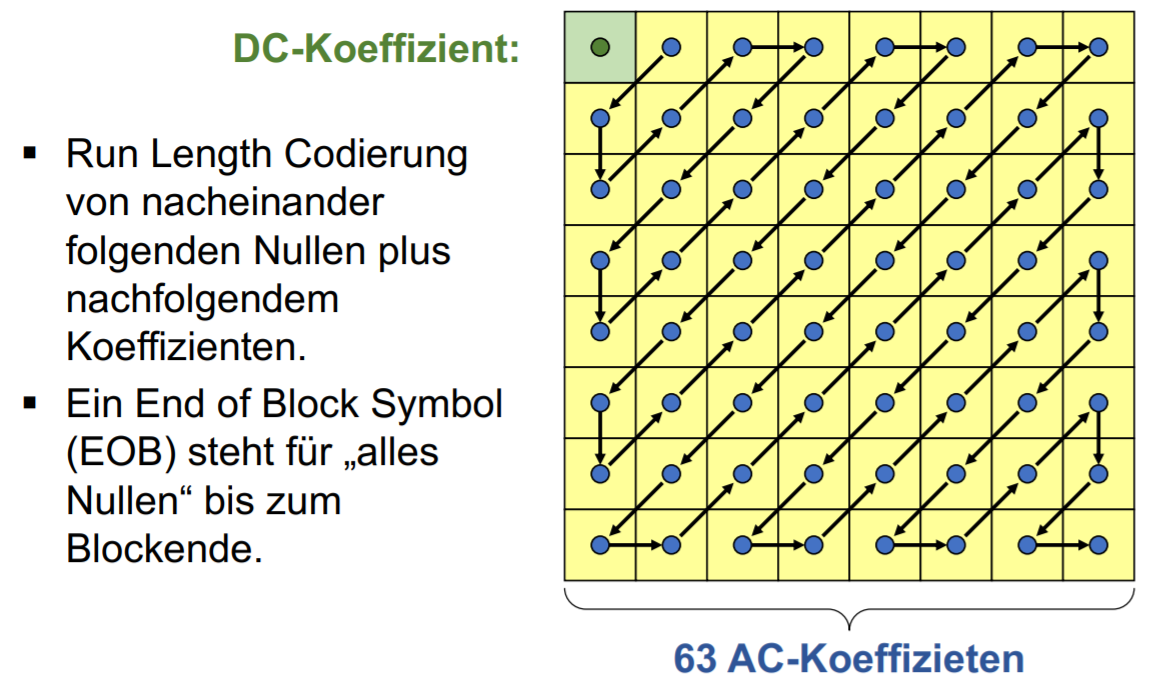
\includegraphics[width=1\linewidth]{images/entropy_encoding.png}
\end{center}

RLE: (DC Wert) (Anzahl Nullen, Koeffizient)...(EOB)

\subsubsection{Dequantisierung}%

\begin{center}
    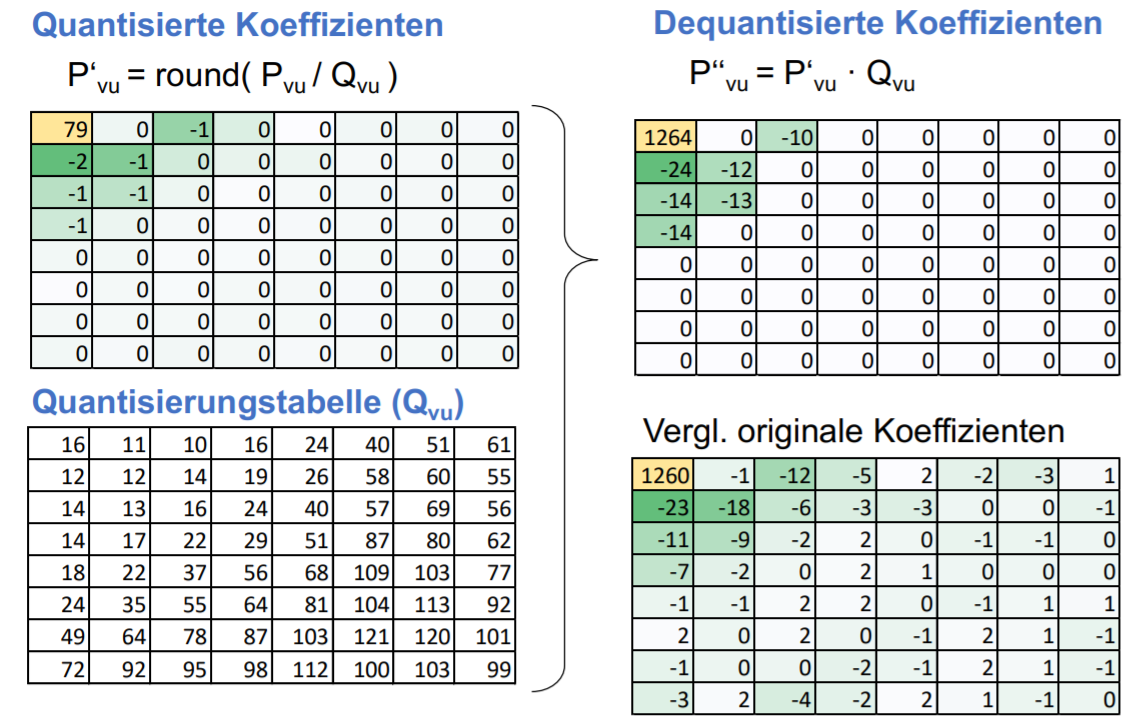
\includegraphics[width=1\linewidth]{images/dequantisierung.png}
\end{center}

\section{Audiocodierung}
\begin{enumerate}
    \item Um ein analoges Audio Signal digitalisieren zu können, muss es abgetastet (sample) und quantisiert werden.
    \item Abtastung bedeutet, dass mit einer bestimmten Abtastfrequenz die Amplitude des Signals gemessen wird.
    \item Quantisierung bedeutet, dass die Amplitude des Signals mit einer bestimmten Anzahl Bits gemessen wird und auf die nächst gelegene Zahl gerundet (quantisiert) wird.
\end{enumerate}

\subsection{Pulse Code Modulation}
\subsubsection{Filterung}
Mit Hilfe eines Filters werden die zu hohen und zu tiefen Frequenzen entfernt. Das Signal wird also auf einen hörbaren Frequenzbereich (20-20kHZ) begrenzt.
\subsubsection{Abtastung}
Die Abtastfrequenz muss mindestens \textbf{doppelt} so gross sein, wir die höchste im analogen Signal vorkommende Frequenz (\textbf{Abtasttheorem von Shannon}).
\subsubsection{Quantisierung}
Die Anzahl Bit, die für die Quantisierung verwendet werden, bestimmt die Anzahl Stufen, welche für die Messung der Amplitude zur Verfügung stehen.
Der Quantisierungsfehler bezeichnet den Fehler, der entsteht wenn die gemessenen Werte gerundet werden.
\subsubsection{Codierung}
Jedem quantisierten Messwert wird ein Wert von einer bestimmten Bitlänge zugeordnet. \textbf{Bitstrom: } Anzahl bits pro Messwert multipliziert mit der Abtastfrequenz.

\subsubsection{Spiegelung}
Bei Eingangssignalen, die grösser sind als die Hälfte der Abtastfrequenz, das "erkannte" Signal an der halben Abtastfrequenz gespiegelt. Bei einer Abtastfrequenz von 8kHz gilt:
\begin{enumerate}
    \item Originalsignal 7kHz -> erkanntes Signal 1kHz
    \item Originalsignal 6kHz -> erkanntes Signal 2kHz
    \item Originalsignal 5kHz -> erkanntes Signal 3kHz
\end{enumerate}

\subsubsection{Quantisierung}%
\textbf{Quantisierungsrauschen: } Differenz Quantisierung <-> Signal. Wird kleiner bei grösser Anzahl verwendeter Bits. Mit jedem Bitanstieg nimmt das Quantisierungsrauschen um 6 dB ab. Jede Bit-Zunahme bedeutet eine Verdoppelung der Anzahl Stufen und damit eine Halbierung des Quantisierungsrauschens.

\begin{center}
    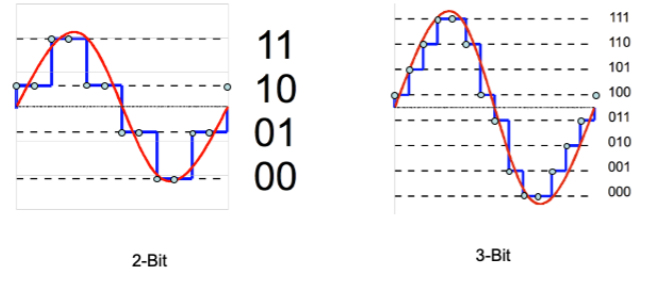
\includegraphics[width=1\linewidth]{images/quantisierungsrauschen.png}
\end{center}

\subsubsection{Lineare Quantisierung}%
Bei einer linearen PCM Codierung wird für jeden Stützwert ein absoluter Wert gemessen und codiert. Dadurch wird bei jedem Stützwert die volle Anzahl Bit für die Quantisierung benötigt.
\begin{center}
    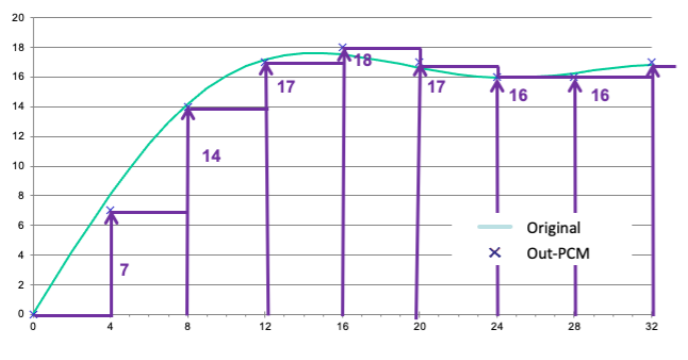
\includegraphics[width=1\linewidth]{images/linearq.png}
\end{center}

\subsubsection{Differential-PCM}%
Bei Differential PCM wird für jeden Stürzwert lediglich die Differenz zum vorherigen Stützwert codiert, was bei Signalfolgen mit geringen Unterschieden - typisch bei digitalen Audiosignalen - zu einer Datenreduktion führt.

\begin{center}
    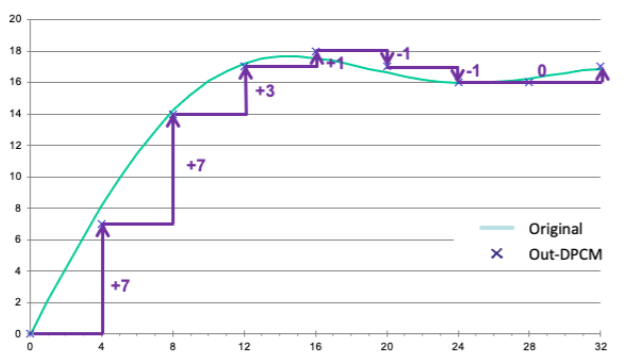
\includegraphics[width=1\linewidth]{images/dpcm.png}
\end{center}

\subsubsection{Adaptive Differential PCM}%
Wird auch Delta Pulse Code Modulation genannt. Wie bei DPCM wird lediglich die Differenz zum vorherigen Stützwert codiert, aber zusätzlich werden nun die Quantisierungsstufen in Abhängigkeit vom Signalverlauf angepasst (adaptiert). Dafür wird ein Korrekturwert K berechnet und nur dieser wird anschliessend übermittelt.
\\
ADPCM ist deshalb ein Codierverfahren mit „Vorhersagefunktion“. Bei der Verarbeitung
des Signals wird versucht, den weiteren Signalverlauf innerhalb des nächsten
Abschnitts vorherzusagen. Für die Quantisierung des Signals im nächsten Zeitschritt
wird so nur die Differenz zwischen vorhergesagtem und realem Signal verwendet. Durch
diese Differenzbildung können so weniger Bits zur Beschreibung des Signals verwendet
werden.
\\
Verfahren: Man misst zuerst die Differenz zum vorherigen Stützwert. Beim nächsten
Stützwert wird die gleiche Differenz (S) noch einmal angewendet und mit dem effektiven
Wert verglichen. Falls der neue Stützwert mit S nicht exakt erreicht wird, wird ein
Korrekturwert K errechnet, um den Wert S so anzupassen, dass die exakte Position
erreicht wird. 
\\
Einerseits können somit gleichbleibende Steigungen mit einer minimalen Anzahl Bit
codiert werden. Andererseits werden zur Beschreibung eines Signals nur die
verhältnismäßig kleinen Korrekturwerte K verwendet, welche mit wenigen Bit
auskommen.
\begin{center}
    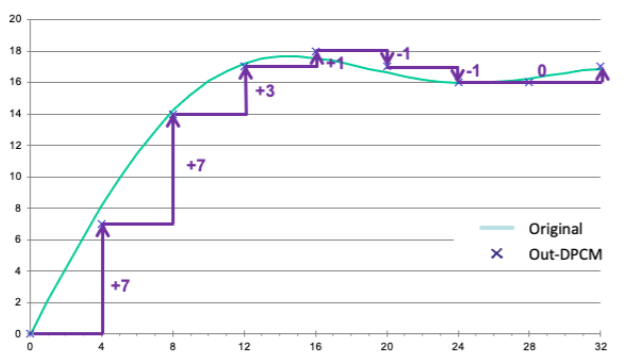
\includegraphics[width=1\linewidth]{images/dpcm.png}
\end{center}

\subsubsection{Linear Prediction Coder LPC}%
\label{ssub:linear_prediction_coder_lpc}

\begin{center}
    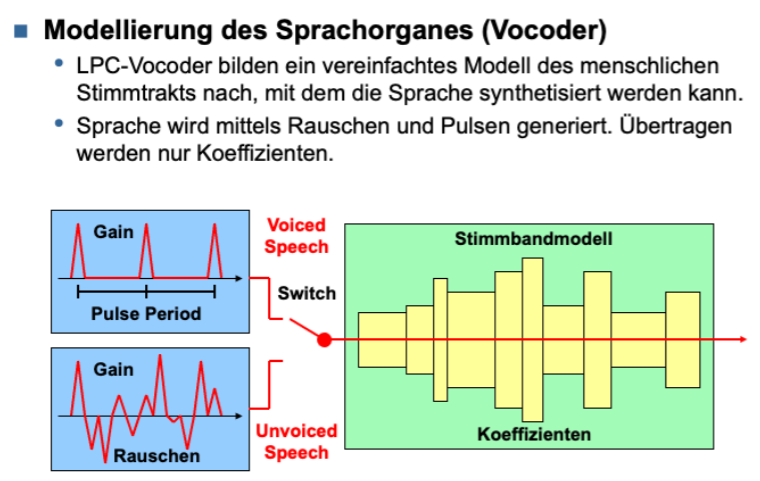
\includegraphics[width=1\linewidth]{images/lpc.png}
\end{center}

\subsection{Wave File Format}%
\label{sub:wave_file_format}

\begin{enumerate}
    \item Containerformat zur digitalen Speicherung von Audiodateien
    \item Basierend auf Microsoft Resource Interchange Format (RIFF)
    \item Wave Dateien enthalten normalerweise keine komprimierten Audiodateien sondern lediglich PCM-Rohdaten
    \item Eine WAVE-Datei enthält vor den Audiodaten einen Header mit Informationen über deren Format
\end{enumerate}

\begin{center}
    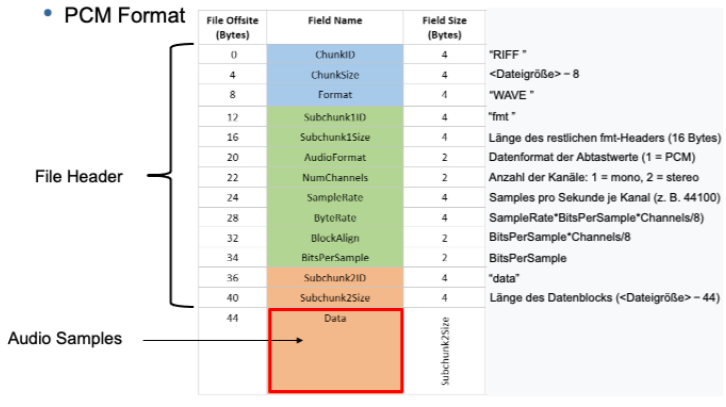
\includegraphics[width=1\linewidth]{images/wave.png}
\end{center}

\begin{center}
    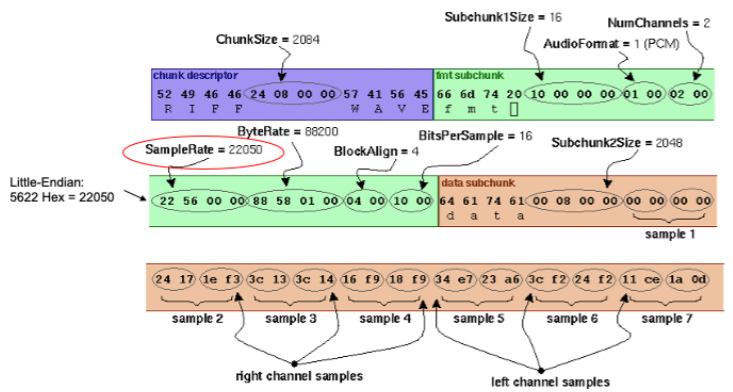
\includegraphics[width=1\linewidth]{images/wavebsp.png}
\end{center}

\subsubsection{Samples}%
\label{ssub:samples}
Die einzelnen Samples $S_i$ für eine gewünschte Frequenz $f$ kann in Abhängigkeit der Abtastrate $R$ und dem Skalierungsfaktor $K$ berechnet werden: $S_i = K \cdot sin(\frac{i \cdot 2 \pi \cdot f}{R})$

Die so erzeugten Samples haben entsprechend ein Intervall von $\frac{2\pi \cdot f}{R}$

\subsubsection{Grösse der Audiodatei}%
\label{ssub:grösse_der_audiodatei}
Header[Byte] + (Abtastfrequenz[Hz] * Dauer[s] + 1) * Auflösung[Byte] * Anzahl Kanäle = [Byte]

\subsection{Schalldruckpegel}%
Schallpegel $L=20 \cdot \log_{10} \frac{p}{p_0}$ Verdoppelung: +6dB.

Der Schalldruckpegel (englisch Sound Pressure Level und oft mit SPL abgekürzt) ist eine
logarithmische Größe zur Beschreibung der Stärke eines Schallereignisses. Der
Schalldruckpegel ist eine berechnete Größe, basierend auf dem Effektivwert des
Schalldrucks.

Der Bezugsschalldruck p0 entspricht der Hörschwelle bei 1kHz und wurde international
normiert auf 0.00002 Pa gesetzt. 

\subsubsection{Menschliche Hörschwelle}%
\label{ssub:menschliche_hörschwelle}

\begin{center}
    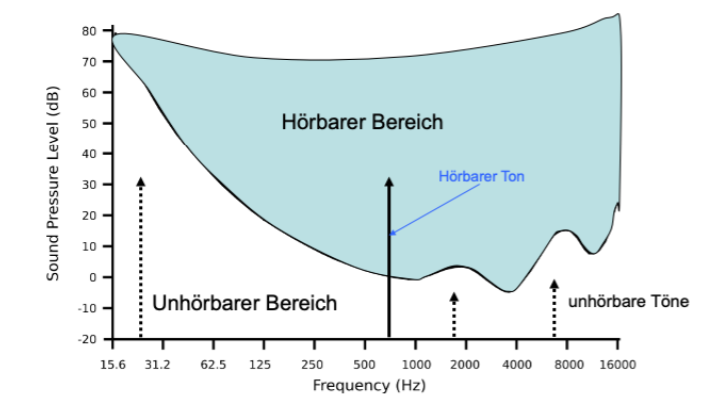
\includegraphics[width=1\linewidth]{images/hoerschwelle.png}
\end{center}

\subsubsection{Maskierung}%
\label{ssub:maskierung}
\begin{enumerate}
    \item Ein lauter Ton kann einen leiseren Ton effektiv maskieren
    \item Je lauter der Ton, desto grösser ist der Frequenzbereich unter- und oberhalb, den er maskieren kann.
    \item Vor-, während und nach einem Ton oder Schallereignis sind leisere Töne nicht hörbar.
\end{enumerate}
\vfill
\subsubsection{Sub-Band Coding}%
\begin{enumerate}
    \item Mehr Bit für die Abtastung -> tieferes Quantisierungs Rauschen
    \item Weniger Bit für die Abtastung -> höheres Quantisierungsrauschen
\end{enumerate}
\begin{center}
    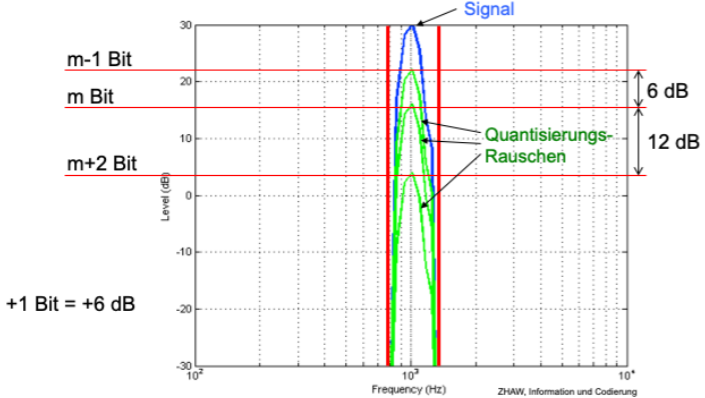
\includegraphics[width=1\linewidth]{images/subband.png}
\end{center}
\begin{center}
    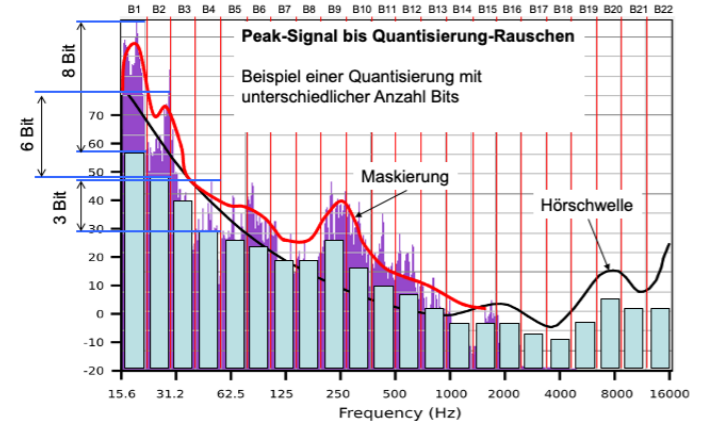
\includegraphics[width=1\linewidth]{images/subband2.png}
\end{center}

\subsection{MPEG Audio}%
\begin{center}
    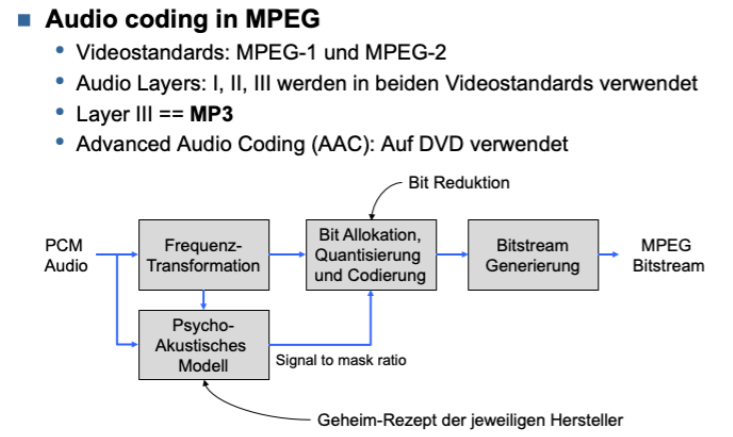
\includegraphics[width=1\linewidth]{images/mpeg.png}
\end{center}
\vfill

    \section{Kanalcodierung}
Ziel: Redundanz hinzufügen

\subsection{Fehlerkorrekturverfahren}
\textbf{Backward Error Correction: } Die Redundanz erlaubt lediglich, Fehler zu erkennen und eine Neuübertragung der Daten anzufordern. \\
\textbf{Forward Error Correction: } Die von der Kanalcodierung hinzugefügte Redundanz reicht, um bei Empfänger Fehler zu korrigieren.

\subsection{Binäre Kanäle}%
Binäre Kanäle können nur die Werte 0 und 1 übertragen. Übertragungsfehler entstehen dadurch, dass ein Bit geflipped wird.

\textbf{$\varepsilon$ ist die Bitfehlerwahrscheinlichkeit (BER Bit Error Ratio)}

\subsubsection{Bitfehlerwahrscheinlichkeit}
Die Bitfehlerwahrscheinlichkeit ε ist eine Eigenschaft des Kanals. \\
Für den symmetrischen Binären Kanal (BSC) gilt:
\begin{enumerate}
    \item Die Fehlerwahrscheinlichkeit ist unabhängig vom Eingangssymbol
    \item Die Wahrscheinlichkeiten $P(y_m|x_n)$ der Übergänge bei gegebenem $x_n$ sind:
\end{enumerate}
\begin{center}
    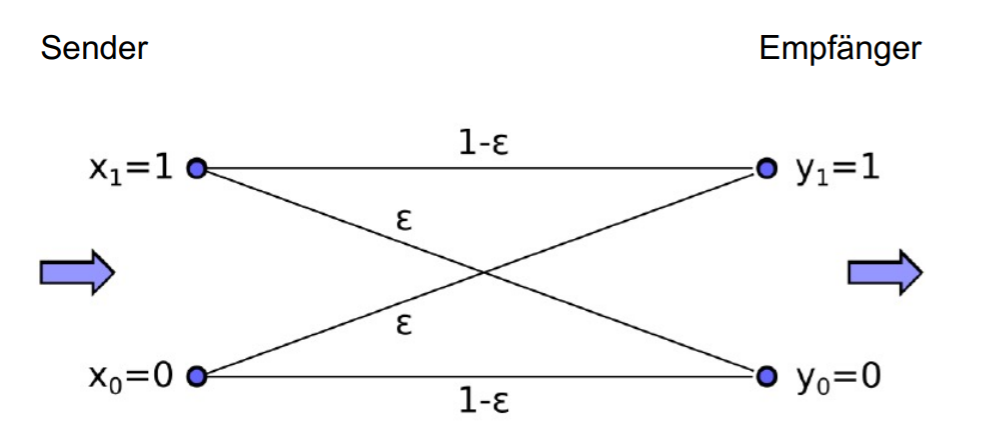
\includegraphics[width=1\linewidth]{images/fehlerwahrscheinlichkeiten.png}
\end{center}
\textbf{Erfolgswahrscheinlichkeit: } $P_{0,N}=\frac{A_N}{A}=(1-\varepsilon)^N$ \\
\textbf{Fehlerwahrscheinlichkeit: } (auf N Datenbits) $1-P_{0,N}=1-(1-\varepsilon)^N$
\begin{center}
    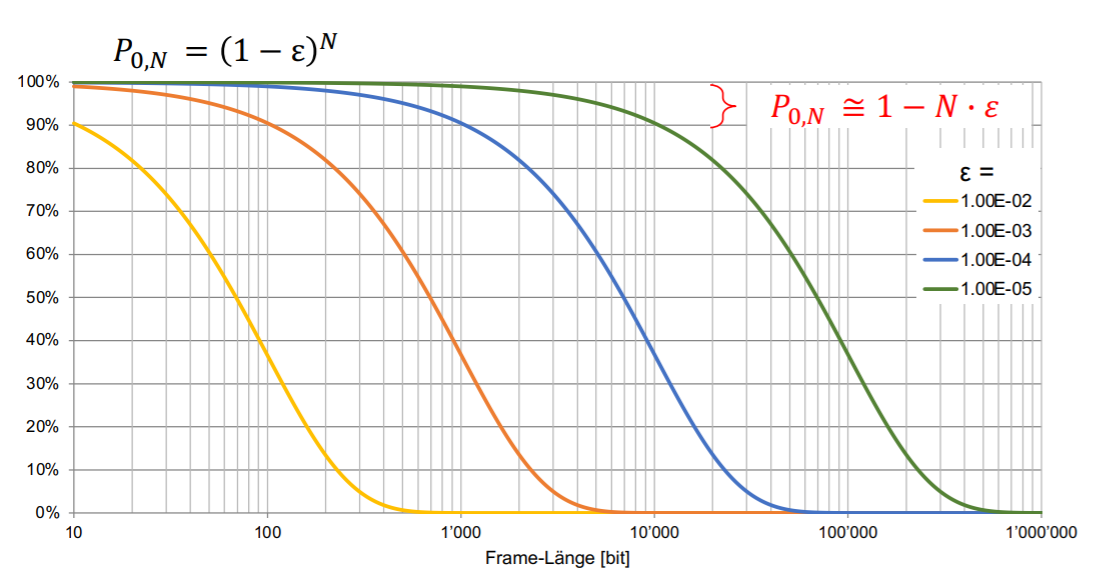
\includegraphics[width=1\linewidth]{images/fehlergraph.png}
\end{center}

\subsubsection{Mehr-Bit-Fehlerwahrscheinlichkeit einer Sequenz}%
Die Wahrscheinlichkeit $P_{F,N}$, dass in einer Sequenz von $N$ Datenbits genau $F$ Bitfehler auftreten, ist:
\[
    P_{F,N} = \binom{N}{F} \cdot \varepsilon^F \cdot (1-\varepsilon)^{N-F}
\]

\begin{center}
    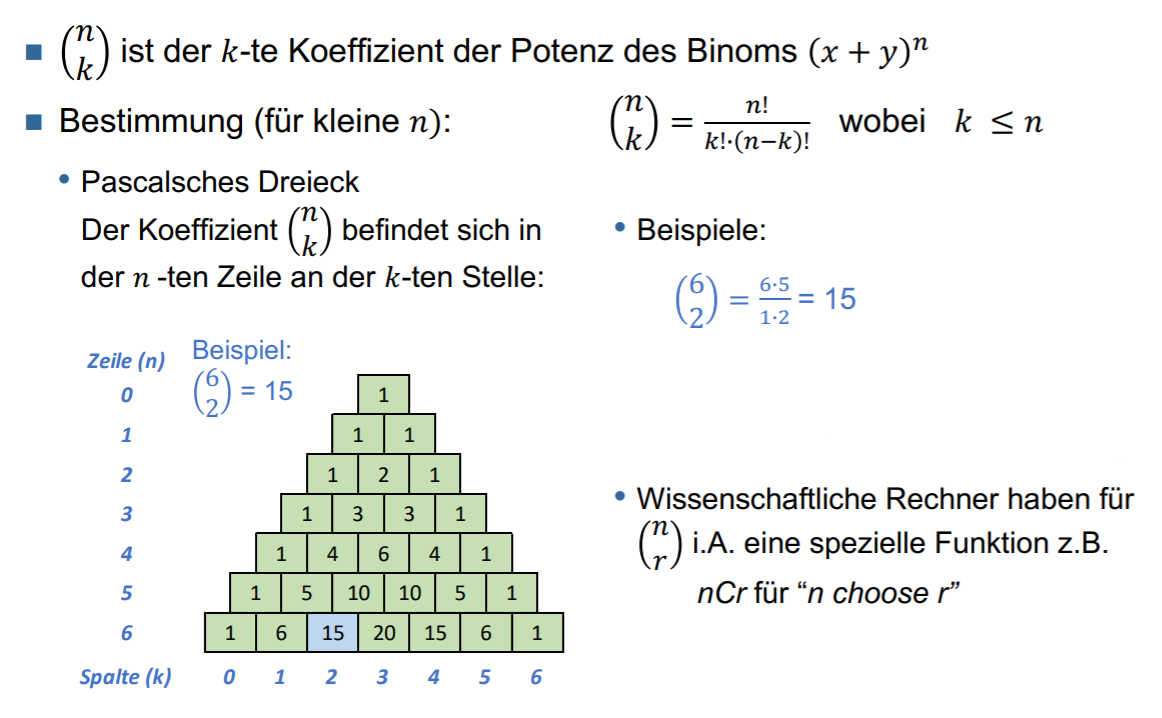
\includegraphics[width=1\linewidth]{images/binominalcoefficient.png}
\end{center}

Für die Wahrscheinlichkeit, dass maximal F Fehler bei einer Übertragung von N Bits auftreten, bilden wir die Summe aller Fälle:
\[
    P_{\leq F, N} = \sum^{F}_{t=0}\binom{N}{t} \cdot \varepsilon^t \cdot (1-\varepsilon)^{N-t}
\]

Restfehlerwahrscheinlichkeit (mehr als F Fehler bei einer Übertragung von N Bits):
\[
    P_{>F,N}=\sum^{N}_{t=F+1}\binom{N}{t} \cdot \varepsilon^t \cdot (1-\varepsilon)^{N-t}
\]

\subsection{Kanalkapazität des BSC}%

Die maximale Kanalkapazität entspricht der Entropie einer binären Quelle: 1bit/Symbol = 1 bit/bit.

\begin{center}
    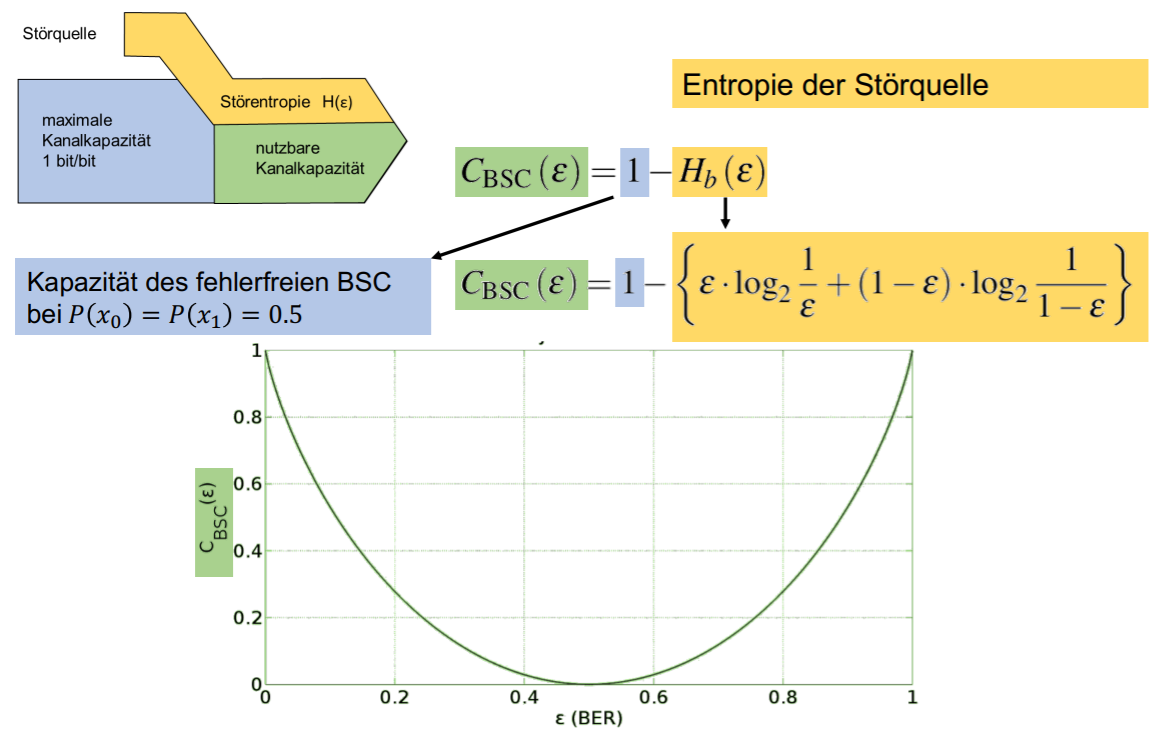
\includegraphics[width=1\linewidth]{images/kanalkapazitaet.png}
\end{center}

\subsubsection{Eingangs- und Ausgangswahrscheinlichkeiten}%

\begin{center}
    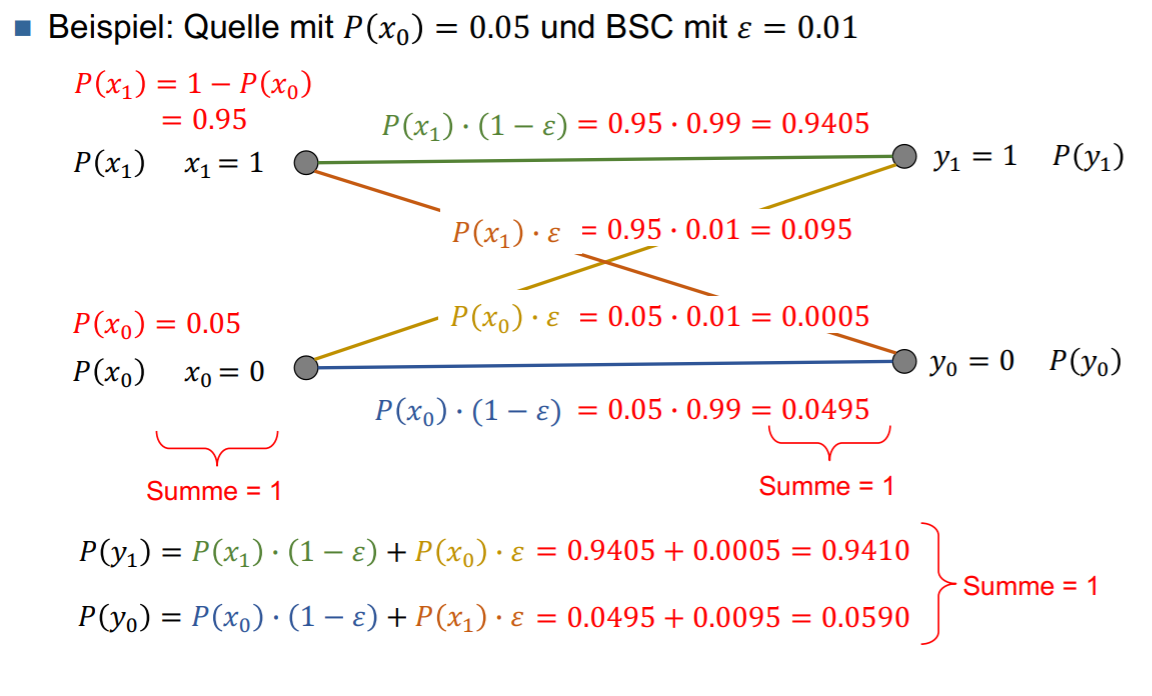
\includegraphics[width=1\linewidth]{images/einauswahrscheinlichkeit.png}
\end{center}

\subsubsection{Entropien eines BSC}%

\begin{center}
    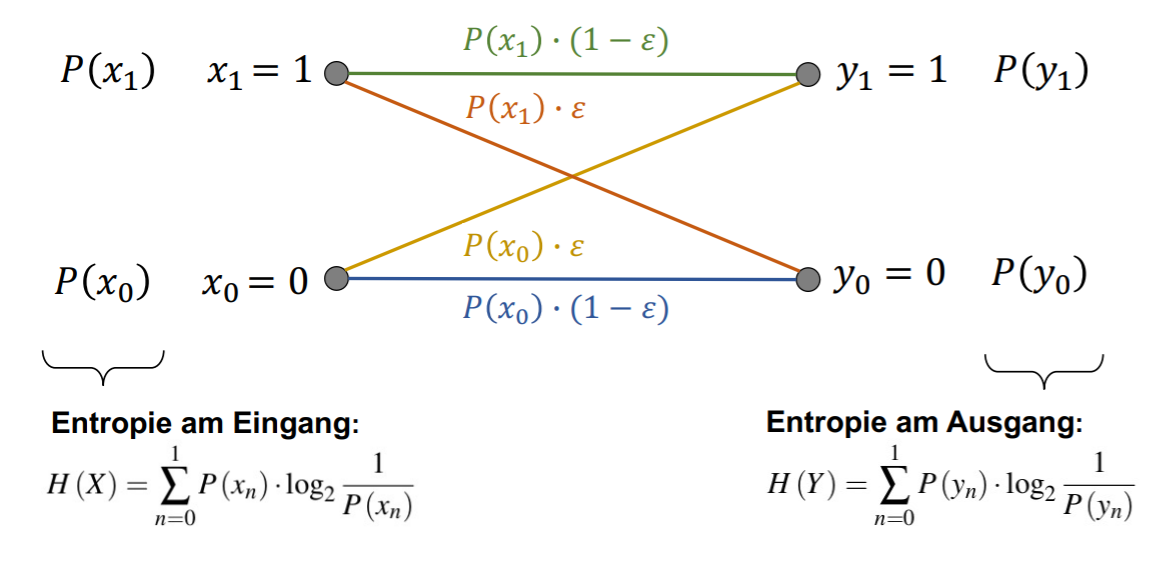
\includegraphics[width=1\linewidth]{images/bscentropy.png}
\end{center}

\subsubsection{Gemeinsame Information}%
Die übertragene Information, die dem Eingang und dem Ausgang gemeinsam ist, kan trotz Fehlern übertragen werden. Sind H(Y) und H(ε) bekannt, folgt für die gemeinsame Information I(X,Y): \textbf{$I(X,Y) = H(Y) - H(\varepsilon) [bit/bit]$}

\subsection{Hamming Distanz}%
\label{sub:hamming_distanz}

Hamming-Distanz ist die Anzahl der wechselnden Bits von einem gültigen Code zum nächsten gültigen Code. Codes mit Hamming-Distanz ≥ 2 erlauben die Erkennung von
Ein- oder Mehr-Bitfehlern.

\begin{center}
    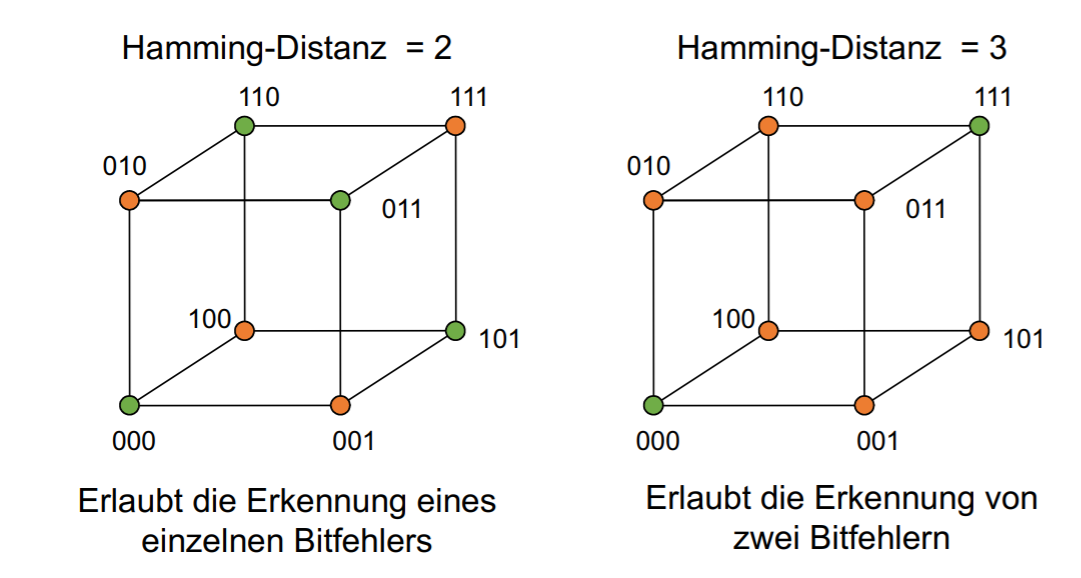
\includegraphics[width=1\linewidth]{images/hammingdist.png}
\end{center}

\subsubsection{Minimale Hamming Distanz}%
\label{ssub:minimale_hamming_distanz}

Die Hamming Distanz $d$ zwischen den Codewörtern ist nicht per se konstant.
Für eine sichere Fehlererkennung oder (später auch Fehlerkorrektur) ist
die minimale Hamming-Distanz $d_{min}(C)$ eines Codes $C$ relevant:
\[
    d_{min}(C)=min d_H (c_j, c_k)
\]

Ein \textbf{perfekter Code} liegt vor, wenn jedes empfangene Wort $w$ genau ein Codewort $c$ hat, zu dem es einen geringsten Hamming-Abstand hat und zu dem es eindeutig zugeordnet werden kann.

\subsubsection{Hamming-Gewicht}%
\label{ssub:hamming_gewicht}

Gibt an, wieviele Einsen das Codewort $c_j$ enthält. Anwendung: Bestimmung der Hamming-Distanz zweier Codewörter.
Dazu bildet man mit einer bitweisen XOR-Operation die Differenz zweier
Codewörter und bestimmt dann davon das Hamming-Gewicht, also die Anzahl
der unterschiedlichen Bits.

\subsection{Binäre Blockcodes}%
\label{sub:binäre_blockcodes}

\begin{center}
    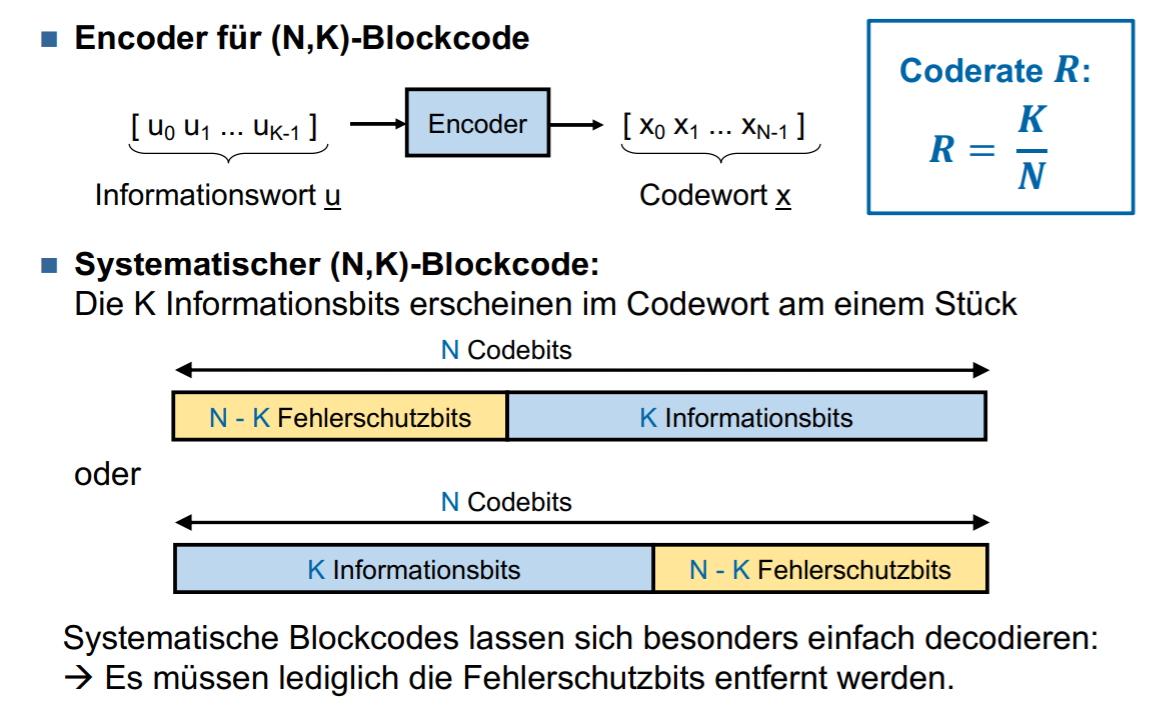
\includegraphics[width=1\linewidth]{images/blockc.png}
\end{center}

\subsubsection{Linearität}%
\label{ssub:linearität}

Bei einem \textbf{linearen (N,K) Blockcode} ist die bitweise Exor-Verknüpfung von 2 beliebigen Codewörtern (inklusive des selben) wieder ein gültiges Codewort.

Bei linearen Blockcodes ist $d_min$ das minimale Hamming-Gewicht.

\subsubsection{Zyklizität}%
\label{ssub:zyklizität}
Die zyklische Verschiebung eines Codeworts gibt wieder ein Codewort.

\subsection{Kanalcodierungstheorem}%
\label{sub:kanalcodierungstheorem}
Möchte man die Restfehlerwahrscheinlichkeit eines Fehlerschutzcodes beliebig klein machen, so muss $R < C$ sein.
\begin{enumerate}
    \item $C$: Kanalkapazität in bit/bit $C_{BSC}=1-H_b(\varepsilon)$
    \item $R$: Coderate in bit/bit $R=\frac{K}{N}$
    \item $R$ muss kleiner als $C$ sein, damit alle Informationen in den nutzbaren Bits Platz haben.
\end{enumerate}

\section{Fehlererkennung}%
\label{sec:fehlererkennung}

Jedes Codewort besteht aus $N$ Bits, wovon $K$ Informationsbits sind und $P$ Prüfbits. $N=K+P$ Mit $N$ Bits gibt es $2^N$ Möglichkeiten für Bitmuster, wovon aber nur $2^K$ gültige Codeworte sind. Die restlichen, ungültigen Bitmuster stehen zur Verfügung, um Fehler zu erkennen.

\subsection{Fehlererkennung mit Parity / Prüfsumme}%
\label{sub:fehlererkennung_mit_parity_prüfsumme}
\begin{enumerate}
    \item Even Parity: Anzahl 1er inkl. Parity-Bit ist gerade
    \item Odd Parity: Anzahl 1er inkl. Parity-Bit ist ungerade
    \item Even Parity und Odd Parity sind gleichwertig, aber nur Even Parity ist linear.
    \item Prüfsumme P = $\sum^{n-1}_{i=0}$ Element[i]
\end{enumerate}

\subsection{1-Bit Polynom-Arithmetik und CRC}%
Bei CRC werden die Bits als Koeffizienten eines Polynoms aufgefasst. \\
\textbf{Beispiel: } Das binäre Datenwort u = (101001) wird zum Polynom U(z):
\[
    U(z) = 1 \cdot z^5 + 0 \cdot z^4 + 1 \cdot z^3 + 0 \cdot z^2 + 0 \cdot z^1 + 1 \cdot z^0 = z^5 \cdot z^3 + 1
\]

Bei der Addition und Subtraktion der Koeffizienten wird die 1-Bit Arithmetik verwendet.

\begin{center}
    \includegraphics[width=1\linewidth]{images/crcm.png}
\end{center}

\begin{enumerate}
    \item CRC-Verfahren wird mathematisch als Modulo-2-Polynomdivision beschrieben, deren Divisionsrest die Prüfbits bildet.
    \item Generator-Polynome(Divisor) werden in der folgenden Form beschrieben: $X^4 + X + 1$, $1 \cdot X^4 + 0 \cdot X^3 + 0 \cdot X^2 + 0 \cdot X^1 + 1 \cdot X^0$ bedeutet 10011b entspricht.
    \item Der gesamte Datenbitstrom wird durch das Generator-Polynom dividiert.
    \item Der Divisionsrest wird angefügt.
    \item Die Hamming-Distanz ist nur abhängig von der Wahl des Generator Polynoms und der Länge der Daten.
\end{enumerate}

\subsubsection{CRC Encoder}%
\label{ssub:crc_encoder}

\begin{center}
    \includegraphics[width=1\linewidth]{images/crcen.png}
\end{center}

\begin{center}
    \includegraphics[width=1\linewidth]{images/crcdec.png}
\end{center}

\subsubsection{CRC Decoder}%
\label{ssub:crc_decoder}

\begin{center}
    \includegraphics[width=1\linewidth]{images/crcdecp.png}
\end{center}

\subsubsection{CRC Implementierung in Hardware}%
\label{ssub:crc_implementierung_in_hardware}

\begin{center}
    \includegraphics[width=1\linewidth]{images/crchard.png}
\end{center}

\subsubsection{CRC Polynomselektion}%
\label{ssub:crc_polynomselektion}

\begin{center}
    \includegraphics[width=1\linewidth]{images/crcpol.png}
\end{center}

\section{Fehlerkorrektur}%
\label{sec:fehlerkorrektur}

Die Anzahl der korrigierbaren Bitfehler (k) ist die abgerundete Hälfte der fehlerbehafteten Zwischencodes:
\[
    k \leq (d_{min} -1)/2
\]

\subsection{Blockcodes}%
\label{sub:blockcodes}

Bei Blockcodes sind bis zu $d_{min}-1$ Fehler pro Codewort erkennbar und $\frac{d_{min}-1}{2}$ Bit Fehler pro Codewort richtig korrigierbar.

\subsubsection{Prüfbits}%
\label{ssub:prüfbits}
Benötigte Prüfbits, um einen Einbitfehler in K Datenbits korrigieren zu können:
\[
    I(p) = \log_{2}(N+1), p \geq \log_2 (K + p + 1)
\]
Näherung: $I(p) \approx I(K+1) = log_2(K+1)$

\subsubsection{Hamming-Codes}%
\label{ssub:hamming_codes}
Codes mit $d_{min} = 3$ und $p = \log_2 (N+1)$ besitzen genau die minimale Anzahl benötigter Prüfbits. \\
Es sind alles perfekte Codes; für alle gilt: $d_H = d_min$ \\
Anhand von $p$ lässt sich $N$, $K$ und die Coderate $R$ berechnen:

\begin{center}
    \includegraphics[width=1\linewidth]{images/hammingcodes.png}
\end{center}

\subsubsection{Lineare Blockcodes - Encoder}%
\label{ssub:lineare_blockcodes}
Hamming-Codes gehören zu den linearen (N,K) Blockcodes. Sie werden durch eine Generatormatrix definiert, die sich aus einer Paritätsmatrix und einer Einheitsmatrix zusammensetzt.

\begin{center}
    \includegraphics[width=1\linewidth]{images/linearbl.png}
\end{center}

Beispiel mit einem (7,4) Hamming-Code:
\[
    \begin{pmatrix}
    1 & 1 & 0 & 1 & 0 & 0 & 0 \\
    0 & 1 & 1 & 0 & 1 & 0 & 0 \\
    1 & 1 & 1 & 0 & 0 & 1 & 0 \\
    1 & 0 & 1 & 0 & 0 & 0 & 1 
    \end{pmatrix}
\]
Das Nutzdatenwort $u_{10} = (1010)$ wird mit der Matrix multipliziert, wodurch das Codewort $0011010$ entsteht. \\
Die Generatormatrix nimmt also Nutzdatenvektoren der Länge $K=4$ auf und produziert daraus Codeworte der Länge $N=7$. \\
Jedes Codewort $c_j$ ist eine Linearkombination von Zeilen der Generatormatrix $G_h$ ist. \\
Die rechten vier Spalten der Generatormatrix $G_h$ bilden eine Einheitsmatrix $I^{4x4}$. Diese Einheitsmatrix bewirkt, dass an der betreffenden Stelle im Codewort $c_j$, also rechtsbündig, der Nutzdatenvektor $u_j$ erscheint. Ein Code mit einer derartigen Generatormatrix ist demnach systematisch und lässt sich besonders leicht decodieren.
\vfill
\subsubsection{Lineare Blockcodes - Decoder}%
\label{ssub:lineare_blockcodes_decoder}

Aus der Generatormatrix wird eine Prüfmatrix gebildet. Schliesslich wird das empfangene Bitmuster mit dieser multipliziert und anschliessend das Syndrom bestimmt.
\[
    s = \underline{\tilde{x}} \cdot \underline{H}^T = (\underline{c}_j + \underline{e}) \cdot \underline{H}^T=\overbrace{\underline{c}_j \cdot \underline{H}^T}^{\text{=0}}+\underline{e} \cdot \underline{H}^T=\underline{e} \cdot \underline{H}^T
\]

Jedes gültige Codewort $\underline{c}_j$ multipliziert mit der Prüfmatrix $\underline{H}^T$ ergibt $0$. Das Symbol ist also gleich dem Produkt von Fehlervektor und Paritätsprüfmatrix.\\

\subsubsection{Bildung der Generatormatrix und Prüfmatrix}%
\label{ssub:bildung_der_generatormatrix}

\begin{enumerate}
    \item Die Generatormatrix setzt sich aus einer Paritätsmatrix und einer Einheitsmatrix zusammen.
    \item Die Paritätsbits müssen voneinander unabhängig sein; jede Spalte muss unterschiedlich sein.
    \item Der Code ist linear. Für die geforderte $d_{min} = 3$ muss jeder Code (ausser dem Null-Code) mindestens 3 Einsen enthalten.
\end{enumerate}

\begin{center}
    \includegraphics[width=1\linewidth]{images/preufmatrix.png}
\end{center}

\begin{center}
    \includegraphics[width=1\linewidth]{images/bilgen.png}
\end{center}

\subsubsection{Blockcode dekodieren - Verfahren}%
\label{ssub:blockcode_dekodieren_verfahren}

\begin{enumerate}
    \item Berechnung des Syndroms: $\underline{s}=\underline{\tilde{c}} \cdot \underline{H}_h^T$
    \item Syndrom bzw. Fehler Tabelle erstellen (Wie bei Codeworten, jede zeile der matrix ist jeweils ein syndrom)
    \item Fehlerkorrektur (Fehlervektor aus Tabelle mit Fehlerhaftem Code addieren): $\hat{c} = \underline{\tilde{c}} + \underline{\hat{e}}$
    \item Decodierung: $\underline{\hat{c}} \implies \underline{\hat{u}}$
\end{enumerate}

\section{Faltungscodes}%
\label{sec:faltungscodes}
\subsection{Zustandsdiagramm}%
\label{sub:zustandsdiagramm}

\begin{center}
\includegraphics[width=1\linewidth]{images/zstfal.png}
\end{center}

\subsection{Hardware Implementierung}%
\label{sub:hardware_im}

\begin{center}
\includegraphics[width=1\linewidth]{images/falthard.png}
\end{center}

\subsection{Freie Distanz}%
\label{sub:freie_distanz}
Bei Faltungscodes spricht man nicht von minmaler Hamming-Distanz, sondern von $d_{free}$ freier Distanz.\\
Da Faltungscodes stets linear sind, gilt auch $d_{free}=w_{min}$. \\

\subsubsection{Anzahl korrigierbarer Fehler}%
\label{ssub:anzahl_korrigierbarer_fehler}
\[
    \frac{d_{free}-1}{2}, N=3 ... 6 \cdot m \text{Bits}
\]

\subsubsection{Optimum free Distance}%
\label{ssub:optimum_free_distance}

\begin{enumerate}
    \item $\gamma$ bezeichnet die Anzahl Generatoren, $m$ die Länge des Schieberegisters resp. die Anzahl zustände des Encoders
    \item Es zeigt sich, dass zu jedem Wertepaar $(\gamma; m)$ eine maximal mögliche freie Distanz gibt.
    \item Codes, die diese freie Distanz erreichen, nennt man Optimum Free Distance Codes.
\end{enumerate}

\begin{center}
\includegraphics[width=1\linewidth]{images/ofdcodes.png}
\end{center}

\subsection{Viterbi Decoder}%
\label{sub:viterbi_decoder}

\begin{center}
\includegraphics[width=1\linewidth]{images/trellis.png}
\end{center}

\begin{enumerate}
    \item Initialisierung: Am Anfang befindet man sich im Startzustand (00) und initialisiert dessen Fehlerwert zu $F=0$
    \item Bei $k=0$ gibt es zwei mögliche Übergänge vom Startzustand aus:
        \begin{itemize}
            \item Bei Eingangsbit $u_0$ = 0 gib es einen Übergang zum Zustand (00). Man vergleicht die Ausgangsbits im Trellis (hier 00) mit den ersten beiden Bits im Bitmuster und notiert die Fehler.
            \item Bei Eingangsbit = 1 findet ein Zustandswechsel zu (10) statt. Auch hier vergleicht man wieder die Ausgangsbits (11) mit den Eingangsbits im Trellis mit den ersten beiden Bits im Bitmuster und notiert die Fehler
        \end{itemize}
    \item Dies wird so weitergeführt für jede Abzweigung. Wenn mehrere Übergänge zu einem Zielzustand führen nimmt man jeweils den mit den wenigsten Bitfehlern. Die Fehler werden dabei laufend addiert! Wenn bei einer Abzweigung ein Fehler von 1 besteht und bei der nächsten ein Fehler von 2, dann notiert man eine 3 und nicht eine zwei.
    \item Um schliesslich die Schätzung für das ursprüngliche Codewort zu finden, läuft man vom Endzustand rückwärts durch den Trellis bis zum Anfang. Dabei nimmt man immer den Weg mit den wenigsten Fehlern.
    \item Schliesslich findet man den Vektor, mit dem man dann von Vorne den Pfad nochmals verfolgen und schliesslich das ursprüngliche Wort herausfinden kann (Tail-Bits beachten).
\end{enumerate}


	\section{Diverses}
\subsection{Zahlencodes}
\begin{center}
    \csvreader[
        separator=semicolon,
        tabular=|c|cccccc|,
        head=true,
        table head=\hline\rotatebox{90}{Binär} & \rotatebox{90}{BCD} & \rotatebox{90}{Excess-3~} & \rotatebox{90}{Aiken} & \rotatebox{90}{4-2-2-1} & \rotatebox{90}{Gray} & \rotatebox{90}{O'Brien}\\\hline,
        table foot = \hline,
        late after line=\csvifoddrow{\\\rowcolor{white}}{\\\rowcolor{primaryheader!15}}
        ]{tables/codes.csv}{
            1=\binary, 
            2=\bcd, 
            3=\excessThree, 
            4=\aiken, 
            5=\ftto, 
            6=\gray, 
            7=\obrien
            }{%
            \binary & \bcd & \excessThree & \aiken & \ftto & \gray & \obrien
    }%
\end{center}
\vfill
\subsection{Gate Varianten}
\begin{center}
    \rotatebox{90}{\includegraphics[width = 120mm]{images/Logic-gate-index.png}}
\end{center}
\vfill
\subsection{Zehnerpotenzen}
\begin{center}
    \renewcommand{\arraystretch}{1.25}
    \rowcolors{2}{primaryheader!15}{white}
    \begin{tabular}{|clc|}
        \hline
        \rowcolor{white}
        Potenz & Präfix & Symbol\\
        \hline
        $10^{-15}$   &   Femto   &   f       \\
        $10^{-12}$   &   Piko    &   p       \\
        $10^{-9}$    &   Nano    &   n       \\
        $10^{-6}$    &   Mikro   &   $\mu$   \\
        $10^{-3}$    &   Milli   &   m       \\
        $10^{-2}$    &   Zenti   &   c       \\
        $10^{-1}$    &   Dezi    &   d       \\
        \hline
        $10^1$     &   Deka    &   da      \\
        $10^2$     &   Hekto   &   h       \\
        $10^3$     &   Kilo    &   k       \\
        $10^6$     &   Mega    &   M       \\
        $10^9$     &   Giga    &   G       \\
        $10^{12}$  &   Tera    &   T       \\
        $10^{15}$  &   Peta    &   P       \\
        \hline
    \end{tabular}
\end{center}

\subsection{Erweiterte Zweierpotenzen}
\begin{center}
    \rowcolors{2}{primaryheader!15}{white}
    \begin{tabular}{|cr||cl|}
        \hline
        \rowcolor{primaryheader!15}$2^{0}$ & $1.0$ & $2^{-0}$ & $ 1.0$ \\ 
        $2^{1}$ & $2.0$ & $2^{-1}$ & $ 0.5$ \\ 
        $2^{2}$ & $4.0$ & $2^{-2}$ & $ 0.25$ \\ 
        $2^{3}$ & $8.0$ & $2^{-3}$ & $ 0.125$ \\ 
        $2^{4}$ & $16.0$ & $2^{-4}$ & $ 0.0625$ \\ 
        $2^{5}$ & $32.0$ & $2^{-5}$ & $ 0.03125$ \\ 
        $2^{6}$ & $64.0$ & $2^{-6}$ & $ 0.015625$ \\ 
        $2^{7}$ & $128.0$ & $2^{-7}$ & $ 0.0078125$ \\ 
        $2^{8}$ & $256.0$ & $2^{-8}$ & $ 0.00390625$ \\ 
        $2^{9}$ & $512.0$ & $2^{-9}$ & $ 0.001953125$ \\ 
        $2^{10}$ & $1024.0$ & $2^{-10}$ & $ 9.765625^{-4}$ \\ 
        $2^{11}$ & $2048.0$ & $2^{-11}$ & $ 4.8828125^{-4}$ \\ 
        $2^{12}$ & $4096.0$ & $2^{-12}$ & $ 2.44140625^{-4}$ \\ 
        \hline                
    \end{tabular}
\end{center}

\end{multicols*}
\begin{flushleft}
    \rowcolors{2}{primaryheader!15}{white}
    \begin{tabular}{|c|c|c||c|c|c||c|c|c||c|c|c|}
        \hline
        \rowcolor{primaryheader!15}\textcolor{numColor}{$0$} & \textcolor{twoColor}{$0$} & $0000~0000$ & \textcolor{numColor}{$64$} & \textcolor{twoColor}{$64$} & $0100~0000$ & \textcolor{numColor}{$128$} & \textcolor{twoColor}{$128$} & $1000~0000$ & \textcolor{numColor}{$192$} & \textcolor{twoColor}{$-64$} & $1100~0000$\\ 
        \textcolor{numColor}{$1$} & \textcolor{twoColor}{$1$} & $0000~0001$ & \textcolor{numColor}{$65$} & \textcolor{twoColor}{$65$} & $0100~0001$ & \textcolor{numColor}{$129$} & \textcolor{twoColor}{$-127$} & $1000~0001$ & \textcolor{numColor}{$193$} & \textcolor{twoColor}{$-63$} & $1100~0001$\\ 
        \textcolor{numColor}{$2$} & \textcolor{twoColor}{$2$} & $0000~0010$ & \textcolor{numColor}{$66$} & \textcolor{twoColor}{$66$} & $0100~0010$ & \cellcolor{secondaryheader!50}\textcolor{numColor}{$130$} & \textcolor{twoColor}{$-126$} & \cellcolor{secondaryheader!50}$1000~0010$ & \textcolor{numColor}{$194$} & \textcolor{twoColor}{$-62$} & $1100~0010$\\ 
        \textcolor{numColor}{$3$} & \textcolor{twoColor}{$3$} & $0000~0011$ & \textcolor{numColor}{$67$} & \textcolor{twoColor}{$67$} & $0100~0011$ & \textcolor{numColor}{$131$} & \textcolor{twoColor}{$-125$} & $1000~0011$ & \textcolor{numColor}{$195$} & \textcolor{twoColor}{$-61$} & $1100~0011$\\ 
        \textcolor{numColor}{$4$} & \textcolor{twoColor}{$4$} & $0000~0100$ & \textcolor{numColor}{$68$} & \textcolor{twoColor}{$68$} & $0100~0100$ & \textcolor{numColor}{$132$} & \textcolor{twoColor}{$-124$} & $1000~0100$ & \textcolor{numColor}{$196$} & \cellcolor{secondaryheader!50}\textcolor{twoColor}{$-60$} & \cellcolor{secondaryheader!50}$1100~0100$\\ 
        \textcolor{numColor}{$5$} & \textcolor{twoColor}{$5$} & $0000~0101$ & \textcolor{numColor}{$69$} & \textcolor{twoColor}{$69$} & $0100~0101$ & \textcolor{numColor}{$133$} & \textcolor{twoColor}{$-123$} & $1000~0101$ & \textcolor{numColor}{$197$} & \textcolor{twoColor}{$-59$} & $1100~0101$\\ 
        \textcolor{numColor}{$6$} & \textcolor{twoColor}{$6$} & $0000~0110$ & \cellcolor{secondaryheader!50}\textcolor{numColor}{$70$} & \cellcolor{secondaryheader!50}\textcolor{twoColor}{$70$} & \cellcolor{secondaryheader!50}$0100~0110$ & \textcolor{numColor}{$134$} & \textcolor{twoColor}{$-122$} & $1000~0110$ & \textcolor{numColor}{$198$} & \textcolor{twoColor}{$-58$} & $1100~0110$\\ 
        \textcolor{numColor}{$7$} & \textcolor{twoColor}{$7$} & $0000~0111$ & \textcolor{numColor}{$71$} & \textcolor{twoColor}{$71$} & $0100~0111$ & \textcolor{numColor}{$135$} & \textcolor{twoColor}{$-121$} & $1000~0111$ & \textcolor{numColor}{$199$} & \textcolor{twoColor}{$-57$} & $1100~0111$\\ 
        \textcolor{numColor}{$8$} & \textcolor{twoColor}{$8$} & $0000~1000$ & \textcolor{numColor}{$72$} & \textcolor{twoColor}{$72$} & $0100~1000$ & \textcolor{numColor}{$136$} & \cellcolor{secondaryheader!50}\textcolor{twoColor}{$-120$} & \cellcolor{secondaryheader!50}$1000~1000$ & \cellcolor{secondaryheader!50}\textcolor{numColor}{$200$} & \textcolor{twoColor}{$-56$} & \cellcolor{secondaryheader!50}$1100~1000$\\ 
        \textcolor{numColor}{$9$} & \textcolor{twoColor}{$9$} & $0000~1001$ & \textcolor{numColor}{$73$} & \textcolor{twoColor}{$73$} & $0100~1001$ & \textcolor{numColor}{$137$} & \textcolor{twoColor}{$-119$} & $1000~1001$ & \textcolor{numColor}{$201$} & \textcolor{twoColor}{$-55$} & $1100~1001$\\ 
        \cellcolor{secondaryheader!50}\textcolor{numColor}{$10$} & \cellcolor{secondaryheader!50}\textcolor{twoColor}{$10$} & \cellcolor{secondaryheader!50}$0000~1010$ & \textcolor{numColor}{$74$} & \textcolor{twoColor}{$74$} & $0100~1010$ & \textcolor{numColor}{$138$} & \textcolor{twoColor}{$-118$} & $1000~1010$ & \textcolor{numColor}{$202$} & \textcolor{twoColor}{$-54$} & $1100~1010$\\ 
        \textcolor{numColor}{$11$} & \textcolor{twoColor}{$11$} & $0000~1011$ & \textcolor{numColor}{$75$} & \textcolor{twoColor}{$75$} & $0100~1011$ & \textcolor{numColor}{$139$} & \textcolor{twoColor}{$-117$} & $1000~1011$ & \textcolor{numColor}{$203$} & \textcolor{twoColor}{$-53$} & $1100~1011$\\ 
        \textcolor{numColor}{$12$} & \textcolor{twoColor}{$12$} & $0000~1100$ & \textcolor{numColor}{$76$} & \textcolor{twoColor}{$76$} & $0100~1100$ & \cellcolor{secondaryheader!50}\textcolor{numColor}{$140$} & \textcolor{twoColor}{$-116$} & \cellcolor{secondaryheader!50}$1000~1100$ & \textcolor{numColor}{$204$} & \textcolor{twoColor}{$-52$} & $1100~1100$\\ 
        \textcolor{numColor}{$13$} & \textcolor{twoColor}{$13$} & $0000~1101$ & \textcolor{numColor}{$77$} & \textcolor{twoColor}{$77$} & $0100~1101$ & \textcolor{numColor}{$141$} & \textcolor{twoColor}{$-115$} & $1000~1101$ & \textcolor{numColor}{$205$} & \textcolor{twoColor}{$-51$} & $1100~1101$\\ 
        \textcolor{numColor}{$14$} & \textcolor{twoColor}{$14$} & $0000~1110$ & \textcolor{numColor}{$78$} & \textcolor{twoColor}{$78$} & $0100~1110$ & \textcolor{numColor}{$142$} & \textcolor{twoColor}{$-114$} & $1000~1110$ & \textcolor{numColor}{$206$} & \cellcolor{secondaryheader!50}\textcolor{twoColor}{$-50$} & \cellcolor{secondaryheader!50}$1100~1110$\\ 
        \textcolor{numColor}{$15$} & \textcolor{twoColor}{$15$} & $0000~1111$ & \textcolor{numColor}{$79$} & \textcolor{twoColor}{$79$} & $0100~1111$ & \textcolor{numColor}{$143$} & \textcolor{twoColor}{$-113$} & $1000~1111$ & \textcolor{numColor}{$207$} & \textcolor{twoColor}{$-49$} & $1100~1111$\\ 
        \textcolor{numColor}{$16$} & \textcolor{twoColor}{$16$} & $0001~0000$ & \cellcolor{secondaryheader!50}\textcolor{numColor}{$80$} & \cellcolor{secondaryheader!50}\textcolor{twoColor}{$80$} & \cellcolor{secondaryheader!50}$0101~0000$ & \textcolor{numColor}{$144$} & \textcolor{twoColor}{$-112$} & $1001~0000$ & \textcolor{numColor}{$208$} & \textcolor{twoColor}{$-48$} & $1101~0000$\\ 
        \textcolor{numColor}{$17$} & \textcolor{twoColor}{$17$} & $0001~0001$ & \textcolor{numColor}{$81$} & \textcolor{twoColor}{$81$} & $0101~0001$ & \textcolor{numColor}{$145$} & \textcolor{twoColor}{$-111$} & $1001~0001$ & \textcolor{numColor}{$209$} & \textcolor{twoColor}{$-47$} & $1101~0001$\\ 
        \textcolor{numColor}{$18$} & \textcolor{twoColor}{$18$} & $0001~0010$ & \textcolor{numColor}{$82$} & \textcolor{twoColor}{$82$} & $0101~0010$ & \textcolor{numColor}{$146$} & \cellcolor{secondaryheader!50}\textcolor{twoColor}{$-110$} & \cellcolor{secondaryheader!50}$1001~0010$ & \cellcolor{secondaryheader!50}\textcolor{numColor}{$210$} & \textcolor{twoColor}{$-46$} & \cellcolor{secondaryheader!50}$1101~0010$\\ 
        \textcolor{numColor}{$19$} & \textcolor{twoColor}{$19$} & $0001~0011$ & \textcolor{numColor}{$83$} & \textcolor{twoColor}{$83$} & $0101~0011$ & \textcolor{numColor}{$147$} & \textcolor{twoColor}{$-109$} & $1001~0011$ & \textcolor{numColor}{$211$} & \textcolor{twoColor}{$-45$} & $1101~0011$\\ 
        \cellcolor{secondaryheader!50}\textcolor{numColor}{$20$} & \cellcolor{secondaryheader!50}\textcolor{twoColor}{$20$} & \cellcolor{secondaryheader!50}$0001~0100$ & \textcolor{numColor}{$84$} & \textcolor{twoColor}{$84$} & $0101~0100$ & \textcolor{numColor}{$148$} & \textcolor{twoColor}{$-108$} & $1001~0100$ & \textcolor{numColor}{$212$} & \textcolor{twoColor}{$-44$} & $1101~0100$\\ 
        \textcolor{numColor}{$21$} & \textcolor{twoColor}{$21$} & $0001~0101$ & \textcolor{numColor}{$85$} & \textcolor{twoColor}{$85$} & $0101~0101$ & \textcolor{numColor}{$149$} & \textcolor{twoColor}{$-107$} & $1001~0101$ & \textcolor{numColor}{$213$} & \textcolor{twoColor}{$-43$} & $1101~0101$\\ 
        \textcolor{numColor}{$22$} & \textcolor{twoColor}{$22$} & $0001~0110$ & \textcolor{numColor}{$86$} & \textcolor{twoColor}{$86$} & $0101~0110$ & \cellcolor{secondaryheader!50}\textcolor{numColor}{$150$} & \textcolor{twoColor}{$-106$} &\cellcolor{secondaryheader!50} $1001~0110$ & \textcolor{numColor}{$214$} & \textcolor{twoColor}{$-42$} & $1101~0110$\\ 
        \textcolor{numColor}{$23$} & \textcolor{twoColor}{$23$} & $0001~0111$ & \textcolor{numColor}{$87$} & \textcolor{twoColor}{$87$} & $0101~0111$ & \textcolor{numColor}{$151$} & \textcolor{twoColor}{$-105$} & $1001~0111$ & \textcolor{numColor}{$215$} & \textcolor{twoColor}{$-41$} & $1101~0111$\\ 
        \textcolor{numColor}{$24$} & \textcolor{twoColor}{$24$} & $0001~1000$ & \textcolor{numColor}{$88$} & \textcolor{twoColor}{$88$} & $0101~1000$ & \textcolor{numColor}{$152$} & \textcolor{twoColor}{$-104$} & $1001~1000$ & \textcolor{numColor}{$216$} & \cellcolor{secondaryheader!50}\textcolor{twoColor}{$-40$} & \cellcolor{secondaryheader!50}$1101~1000$\\ 
        \textcolor{numColor}{$25$} & \textcolor{twoColor}{$25$} & $0001~1001$ & \textcolor{numColor}{$89$} & \textcolor{twoColor}{$89$} & $0101~1001$ & \textcolor{numColor}{$153$} & \textcolor{twoColor}{$-103$} & $1001~1001$ & \textcolor{numColor}{$217$} & \textcolor{twoColor}{$-39$} & $1101~1001$\\ 
        \textcolor{numColor}{$26$} & \textcolor{twoColor}{$26$} & $0001~1010$ & \cellcolor{secondaryheader!50}\textcolor{numColor}{$90$} & \cellcolor{secondaryheader!50}\textcolor{twoColor}{$90$} & \cellcolor{secondaryheader!50}$0101~1010$ & \textcolor{numColor}{$154$} & \textcolor{twoColor}{$-102$} & $1001~1010$ & \textcolor{numColor}{$218$} & \textcolor{twoColor}{$-38$} & $1101~1010$\\ 
        \textcolor{numColor}{$27$} & \textcolor{twoColor}{$27$} & $0001~1011$ & \textcolor{numColor}{$91$} & \textcolor{twoColor}{$91$} & $0101~1011$ & \textcolor{numColor}{$155$} & \textcolor{twoColor}{$-101$} & $1001~1011$ & \textcolor{numColor}{$219$} & \textcolor{twoColor}{$-37$} & $1101~1011$\\ 
        \textcolor{numColor}{$28$} & \textcolor{twoColor}{$28$} & $0001~1100$ & \textcolor{numColor}{$92$} & \textcolor{twoColor}{$92$} & $0101~1100$ & \textcolor{numColor}{$156$} & \cellcolor{secondaryheader!50}\textcolor{twoColor}{$-100$} & \cellcolor{secondaryheader!50}$1001~1100$ & \cellcolor{secondaryheader!50}\textcolor{numColor}{$220$} & \textcolor{twoColor}{$-36$} & \cellcolor{secondaryheader!50}$1101~1100$\\ 
        \textcolor{numColor}{$29$} & \textcolor{twoColor}{$29$} & $0001~1101$ & \textcolor{numColor}{$93$} & \textcolor{twoColor}{$93$} & $0101~1101$ & \textcolor{numColor}{$157$} & \textcolor{twoColor}{$-99$} & $1001~1101$ & \textcolor{numColor}{$221$} & \textcolor{twoColor}{$-35$} & $1101~1101$\\ 
        \cellcolor{secondaryheader!50}\textcolor{numColor}{$30$} & \cellcolor{secondaryheader!50}\textcolor{twoColor}{$30$} & \cellcolor{secondaryheader!50}$0001~1110$ & \textcolor{numColor}{$94$} & \textcolor{twoColor}{$94$} & $0101~1110$ & \textcolor{numColor}{$158$} & \textcolor{twoColor}{$-98$} & $1001~1110$ & \textcolor{numColor}{$222$} & \textcolor{twoColor}{$-34$} & $1101~1110$\\ 
        \textcolor{numColor}{$31$} & \textcolor{twoColor}{$31$} & $0001~1111$ & \textcolor{numColor}{$95$} & \textcolor{twoColor}{$95$} & $0101~1111$ & \textcolor{numColor}{$159$} & \textcolor{twoColor}{$-97$} & $1001~1111$ & \textcolor{numColor}{$223$} & \textcolor{twoColor}{$-33$} & $1101~1111$\\ 
        \textcolor{numColor}{$32$} & \textcolor{twoColor}{$32$} & $0010~0000$ & \textcolor{numColor}{$96$} & \textcolor{twoColor}{$96$} & $0110~0000$ & \cellcolor{secondaryheader!50}\textcolor{numColor}{$160$} & \textcolor{twoColor}{$-96$} & \cellcolor{secondaryheader!50}$1010~0000$ & \textcolor{numColor}{$224$} & \textcolor{twoColor}{$-32$} & $1110~0000$\\ 
        \textcolor{numColor}{$33$} & \textcolor{twoColor}{$33$} & $0010~0001$ & \textcolor{numColor}{$97$} & \textcolor{twoColor}{$97$} & $0110~0001$ & \textcolor{numColor}{$161$} & \textcolor{twoColor}{$-95$} & $1010~0001$ & \textcolor{numColor}{$225$} & \textcolor{twoColor}{$-31$} & $1110~0001$\\ 
        \textcolor{numColor}{$34$} & \textcolor{twoColor}{$34$} & $0010~0010$ & \textcolor{numColor}{$98$} & \textcolor{twoColor}{$98$} & $0110~0010$ & \textcolor{numColor}{$162$} & \textcolor{twoColor}{$-94$} & $1010~0010$ & \textcolor{numColor}{$226$} & \cellcolor{secondaryheader!50}\textcolor{twoColor}{$-30$} & \cellcolor{secondaryheader!50}$1110~0010$\\ 
        \textcolor{numColor}{$35$} & \textcolor{twoColor}{$35$} & $0010~0011$ & \textcolor{numColor}{$99$} & \textcolor{twoColor}{$99$} & $0110~0011$ & \textcolor{numColor}{$163$} & \textcolor{twoColor}{$-93$} & $1010~0011$ & \textcolor{numColor}{$227$} & \textcolor{twoColor}{$-29$} & $1110~0011$\\ 
        \textcolor{numColor}{$36$} & \textcolor{twoColor}{$36$} & $0010~0100$ & \cellcolor{secondaryheader!50}\textcolor{numColor}{$100$} & \cellcolor{secondaryheader!50}\textcolor{twoColor}{$100$} & \cellcolor{secondaryheader!50}$0110~0100$ & \textcolor{numColor}{$164$} & \textcolor{twoColor}{$-92$} & $1010~0100$ & \textcolor{numColor}{$228$} & \textcolor{twoColor}{$-28$} & $1110~0100$\\ 
        \textcolor{numColor}{$37$} & \textcolor{twoColor}{$37$} & $0010~0101$ & \textcolor{numColor}{$101$} & \textcolor{twoColor}{$101$} & $0110~0101$ & \textcolor{numColor}{$165$} & \textcolor{twoColor}{$-91$} & $1010~0101$ & \textcolor{numColor}{$229$} & \textcolor{twoColor}{$-27$} & $1110~0101$\\ 
        \textcolor{numColor}{$38$} & \textcolor{twoColor}{$38$} & $0010~0110$ & \textcolor{numColor}{$102$} & \textcolor{twoColor}{$102$} & $0110~0110$ & \textcolor{numColor}{$166$} & \cellcolor{secondaryheader!50}\textcolor{twoColor}{$-90$} & \cellcolor{secondaryheader!50}$1010~0110$ & \cellcolor{secondaryheader!50}\textcolor{numColor}{$230$} & \textcolor{twoColor}{$-26$} & \cellcolor{secondaryheader!50}$1110~0110$\\ 
        \textcolor{numColor}{$39$} & \textcolor{twoColor}{$39$} & $0010~0111$ & \textcolor{numColor}{$103$} & \textcolor{twoColor}{$103$} & $0110~0111$ & \textcolor{numColor}{$167$} & \textcolor{twoColor}{$-89$} & $1010~0111$ & \textcolor{numColor}{$231$} & \textcolor{twoColor}{$-25$} & $1110~0111$\\ 
        \cellcolor{secondaryheader!50}\textcolor{numColor}{$40$} & \cellcolor{secondaryheader!50}\textcolor{twoColor}{$40$} & \cellcolor{secondaryheader!50}$0010~1000$ & \textcolor{numColor}{$104$} & \textcolor{twoColor}{$104$} & $0110~1000$ & \textcolor{numColor}{$168$} & \textcolor{twoColor}{$-88$} & $1010~1000$ & \textcolor{numColor}{$232$} & \textcolor{twoColor}{$-24$} & $1110~1000$\\ 
        \textcolor{numColor}{$41$} & \textcolor{twoColor}{$41$} & $0010~1001$ & \textcolor{numColor}{$105$} & \textcolor{twoColor}{$105$} & $0110~1001$ & \textcolor{numColor}{$169$} & \textcolor{twoColor}{$-87$} & $1010~1001$ & \textcolor{numColor}{$233$} & \textcolor{twoColor}{$-23$} & $1110~1001$\\ 
        \textcolor{numColor}{$42$} & \textcolor{twoColor}{$42$} & $0010~1010$ & \textcolor{numColor}{$106$} & \textcolor{twoColor}{$106$} & $0110~1010$ & \cellcolor{secondaryheader!50}\textcolor{numColor}{$170$} & \textcolor{twoColor}{$-86$} & \cellcolor{secondaryheader!50}$1010~1010$ & \textcolor{numColor}{$234$} & \textcolor{twoColor}{$-22$} & $1110~1010$\\ 
        \textcolor{numColor}{$43$} & \textcolor{twoColor}{$43$} & $0010~1011$ & \textcolor{numColor}{$107$} & \textcolor{twoColor}{$107$} & $0110~1011$ & \textcolor{numColor}{$171$} & \textcolor{twoColor}{$-85$} & $1010~1011$ & \textcolor{numColor}{$235$} & \textcolor{twoColor}{$-21$} & $1110~1011$\\ 
        \textcolor{numColor}{$44$} & \textcolor{twoColor}{$44$} & $0010~1100$ & \textcolor{numColor}{$108$} & \textcolor{twoColor}{$108$} & $0110~1100$ & \textcolor{numColor}{$172$} & \textcolor{twoColor}{$-84$} & $1010~1100$ & \textcolor{numColor}{$236$} & \cellcolor{secondaryheader!50}\textcolor{twoColor}{$-20$} & \cellcolor{secondaryheader!50}$1110~1100$\\ 
        \textcolor{numColor}{$45$} & \textcolor{twoColor}{$45$} & $0010~1101$ & \textcolor{numColor}{$109$} & \textcolor{twoColor}{$109$} & $0110~1101$ & \textcolor{numColor}{$173$} & \textcolor{twoColor}{$-83$} & $1010~1101$ & \textcolor{numColor}{$237$} & \textcolor{twoColor}{$-19$} & $1110~1101$\\ 
        \textcolor{numColor}{$46$} & \textcolor{twoColor}{$46$} & $0010~1110$ & \cellcolor{secondaryheader!50}\textcolor{numColor}{$110$} & \cellcolor{secondaryheader!50}\textcolor{twoColor}{$110$} & \cellcolor{secondaryheader!50}$0110~1110$ & \textcolor{numColor}{$174$} & \textcolor{twoColor}{$-82$} & $1010~1110$ & \textcolor{numColor}{$238$} & \textcolor{twoColor}{$-18$} & $1110~1110$\\ 
        \textcolor{numColor}{$47$} & \textcolor{twoColor}{$47$} & $0010~1111$ & \textcolor{numColor}{$111$} & \textcolor{twoColor}{$111$} & $0110~1111$ & \textcolor{numColor}{$175$} & \textcolor{twoColor}{$-81$} & $1010~1111$ & \textcolor{numColor}{$239$} & \textcolor{twoColor}{$-17$} & $1110~1111$\\ 
        \textcolor{numColor}{$48$} & \textcolor{twoColor}{$48$} & $0011~0000$ & \textcolor{numColor}{$112$} & \textcolor{twoColor}{$112$} & $0111~0000$ & \textcolor{numColor}{$176$} & \cellcolor{secondaryheader!50}\textcolor{twoColor}{$-80$} & \cellcolor{secondaryheader!50}$1011~0000$ & \cellcolor{secondaryheader!50}\textcolor{numColor}{$240$} & \textcolor{twoColor}{$-16$} & \cellcolor{secondaryheader!50}$1111~0000$\\ 
        \textcolor{numColor}{$49$} & \textcolor{twoColor}{$49$} & $0011~0001$ & \textcolor{numColor}{$113$} & \textcolor{twoColor}{$113$} & $0111~0001$ & \textcolor{numColor}{$177$} & \textcolor{twoColor}{$-79$} & $1011~0001$ & \textcolor{numColor}{$241$} & \textcolor{twoColor}{$-15$} & $1111~0001$\\ 
        \cellcolor{secondaryheader!50}\textcolor{numColor}{$50$} & \cellcolor{secondaryheader!50}\textcolor{twoColor}{$50$} & \cellcolor{secondaryheader!50}$0011~0010$ & \textcolor{numColor}{$114$} & \textcolor{twoColor}{$114$} & $0111~0010$ & \textcolor{numColor}{$178$} & \textcolor{twoColor}{$-78$} & $1011~0010$ & \textcolor{numColor}{$242$} & \textcolor{twoColor}{$-14$} & $1111~0010$\\ 
        \textcolor{numColor}{$51$} & \textcolor{twoColor}{$51$} & $0011~0011$ & \textcolor{numColor}{$115$} & \textcolor{twoColor}{$115$} & $0111~0011$ & \textcolor{numColor}{$179$} & \textcolor{twoColor}{$-77$} & $1011~0011$ & \textcolor{numColor}{$243$} & \textcolor{twoColor}{$-13$} & $1111~0011$\\ 
        \textcolor{numColor}{$52$} & \textcolor{twoColor}{$52$} & $0011~0100$ & \textcolor{numColor}{$116$} & \textcolor{twoColor}{$116$} & $0111~0100$ & \cellcolor{secondaryheader!50}\textcolor{numColor}{$180$} & \textcolor{twoColor}{$-76$} & \cellcolor{secondaryheader!50}$1011~0100$ & \textcolor{numColor}{$244$} & \textcolor{twoColor}{$-12$} & $1111~0100$\\ 
        \textcolor{numColor}{$53$} & \textcolor{twoColor}{$53$} & $0011~0101$ & \textcolor{numColor}{$117$} & \textcolor{twoColor}{$117$} & $0111~0101$ & \textcolor{numColor}{$181$} & \textcolor{twoColor}{$-75$} & $1011~0101$ & \textcolor{numColor}{$245$} & \textcolor{twoColor}{$-11$} & $1111~0101$\\ 
        \textcolor{numColor}{$54$} & \textcolor{twoColor}{$54$} & $0011~0110$ & \textcolor{numColor}{$118$} & \textcolor{twoColor}{$118$} & $0111~0110$ & \textcolor{numColor}{$182$} & \textcolor{twoColor}{$-74$} & $1011~0110$ & \textcolor{numColor}{$246$} & \cellcolor{secondaryheader!50}\textcolor{twoColor}{$-10$} & \cellcolor{secondaryheader!50}$1111~0110$\\ 
        \textcolor{numColor}{$55$} & \textcolor{twoColor}{$55$} & $0011~0111$ & \textcolor{numColor}{$119$} & \textcolor{twoColor}{$119$} & $0111~0111$ & \textcolor{numColor}{$183$} & \textcolor{twoColor}{$-73$} & $1011~0111$ & \textcolor{numColor}{$247$} & \textcolor{twoColor}{$-9$} & $1111~0111$\\ 
        \textcolor{numColor}{$56$} & \textcolor{twoColor}{$56$} & $0011~1000$ & \cellcolor{secondaryheader!50}\textcolor{numColor}{$120$} & \cellcolor{secondaryheader!50}\textcolor{twoColor}{$120$} & \cellcolor{secondaryheader!50}$0111~1000$ & \textcolor{numColor}{$184$} & \textcolor{twoColor}{$-72$} & $1011~1000$ & \textcolor{numColor}{$248$} & \textcolor{twoColor}{$-8$} & $1111~1000$\\ 
        \textcolor{numColor}{$57$} & \textcolor{twoColor}{$57$} & $0011~1001$ & \textcolor{numColor}{$121$} & \textcolor{twoColor}{$121$} & $0111~1001$ & \textcolor{numColor}{$185$} & \textcolor{twoColor}{$-71$} & $1011~1001$ & \textcolor{numColor}{$249$} & \textcolor{twoColor}{$-7$} & $1111~1001$\\ 
        \textcolor{numColor}{$58$} & \textcolor{twoColor}{$58$} & $0011~1010$ & \textcolor{numColor}{$122$} & \textcolor{twoColor}{$122$} & $0111~1010$ & \textcolor{numColor}{$186$} & \cellcolor{secondaryheader!50}\textcolor{twoColor}{$-70$} & \cellcolor{secondaryheader!50}$1011~1010$ & \cellcolor{secondaryheader!50}\textcolor{numColor}{$250$} & \textcolor{twoColor}{$-6$} & \cellcolor{secondaryheader!50}$1111~1010$\\ 
        \textcolor{numColor}{$59$} & \textcolor{twoColor}{$59$} & $0011~1011$ & \textcolor{numColor}{$123$} & \textcolor{twoColor}{$123$} & $0111~1011$ & \textcolor{numColor}{$187$} & \textcolor{twoColor}{$-69$} & $1011~1011$ & \textcolor{numColor}{$251$} & \textcolor{twoColor}{$-5$} & $1111~1011$\\ 
        \cellcolor{secondaryheader!50}\textcolor{numColor}{$60$} & \cellcolor{secondaryheader!50}\textcolor{twoColor}{$60$} & \cellcolor{secondaryheader!50}$0011~1100$ & \textcolor{numColor}{$124$} & \textcolor{twoColor}{$124$} & $0111~1100$ & \textcolor{numColor}{$188$} & \textcolor{twoColor}{$-68$} & $1011~1100$ & \textcolor{numColor}{$252$} & \textcolor{twoColor}{$-4$} & $1111~1100$\\ 
        \textcolor{numColor}{$61$} & \textcolor{twoColor}{$61$} & $0011~1101$ & \textcolor{numColor}{$125$} & \textcolor{twoColor}{$125$} & $0111~1101$ & \textcolor{numColor}{$189$} & \textcolor{twoColor}{$-67$} & $1011~1101$ & \textcolor{numColor}{$253$} & \textcolor{twoColor}{$-3$} & $1111~1101$\\ 
        \textcolor{numColor}{$62$} & \textcolor{twoColor}{$62$} & $0011~1110$ & \textcolor{numColor}{$126$} & \textcolor{twoColor}{$126$} & $0111~1110$ & \cellcolor{secondaryheader!50}\textcolor{numColor}{$190$} & \textcolor{twoColor}{$-66$} & \cellcolor{secondaryheader!50}$1011~1110$ & \textcolor{numColor}{$254$} & \textcolor{twoColor}{$-2$} & $1111~1110$\\ 
        \textcolor{numColor}{$63$} & \textcolor{twoColor}{$63$} & $0011~1111$ & \textcolor{numColor}{$127$} & \textcolor{twoColor}{$127$} & $0111~1111$ & \textcolor{numColor}{$191$} & \textcolor{twoColor}{$-65$} & $1011~1111$ & \textcolor{numColor}{$255$} & \textcolor{twoColor}{$-1$} & $1111~1111$\\ 
        \hline
    \end{tabular}
\end{flushleft}
\end{document}
